\documentclass{article}
\usepackage[a4paper, left=15mm, top=20mm, right=15mm,bottom=20mm]{geometry}
\usepackage{amsmath, amssymb, amsfonts}
\usepackage{fancyhdr}
\usepackage{graphicx}
\graphicspath{ {./images/} }
\usepackage{float}
\usepackage{hyperref}
\usepackage{lscape}
\usepackage{multirow}

\pagestyle{fancy}
\fancyhf{}
\lhead{EC1101E}
\rhead{claudeonrs}
\rfoot{\thepage}
\usepackage{amsmath, amssymb, amsfonts, listings}
\usepackage{xcolor}
\usepackage{enumitem}
\setlist[itemize]{noitemsep, topsep=0pt}
\setlist[enumerate]{noitemsep, topsep=0pt}
\setlist[description]{noitemsep, topsep=0pt}


%New colors defined below
\definecolor{codegreen}{rgb}{0,0.6,0.4}
\definecolor{codegray}{rgb}{0.5,0.5,0.5}
\definecolor{codepurple}{rgb}{0.58,0,0.82}
\definecolor{backcolour}{rgb}{0.95,0.95,0.92}
\definecolor{commentgreen}{rgb}{0.4,0.8,0.6}
%Code listing style named "mystyle"
\lstdefinestyle{mystyle}{
  backgroundcolor=\color{backcolour},
  commentstyle=\color{red},
  keywordstyle=\color{blue},
  numberstyle=\tiny\color{codegray},
  stringstyle=\color{codegreen},
  basicstyle=\ttfamily,
  breakatwhitespace=false,
  breaklines=true,
  captionpos=b,
  keepspaces=true,
  numbers=left,
  numbersep=5pt,
  showspaces=false,
  showstringspaces=false,
  showtabs=false,
  tabsize=2
}

%"mystyle" code listing set
\lstset{style=mystyle}

\title{No Title}
\author{Claudeon R Susanto}
\date{}
\usepackage[T1]{fontenc}
\usepackage[utf8]{inputenc}
\usepackage[english]{babel}
\usepackage{lmodern}

\renewcommand{\familydefault}{\sfdefault}   % Supprime le serif (dyslexie)
\usepackage[font=sf, labelfont={sf}]{caption}
\usepackage{multicol}
\usepackage{makecell}
\renewcommand\theadalign{bc}
\renewcommand\theadfont{\bfseries}
\renewcommand\theadgape{\Gape[4pt]}
\renewcommand\cellgape{\Gape[4pt]}

\renewcommand\thesubsection{\thesection.\arabic{subsection}}
\setlength{\columnseprule}{1pt}




% own commands
\newcommand{\eg}[0]{\textit{e.g. }}
\newcommand{\ie}[0]{\textit{i.e. }}
\newcommand{\impt}[0]{\textcolor{red}{\textbf{[IMPT] }}}


\begin{document}
%\maketitle
\fontfamily{lmss}\selectfont
\begin{multicols}{2}
\section{Introduction to Economic Analysis}
\subsection{Scarcity}
\textbf{Scarce}: Quantity of resources lower than demand, hence insufficient to satisfv needs and wants\\
\textbf{Resources}: CELL (Capital - physical and human capital, Entrepreneurship, Land, Labour)\\


\textbf{What is Economics?}: study of \underline{choice} under \underline{scarcity}
\begin{itemize}
	\item How \underline{people} decide how much to work, what to buy, how much to save, how to invest, etc. given budget and costs
	\item How \underline{firms} decide how much to produce, how many workers to hire, etc. given available budget and costs
	\item How \underline{society} decides how to allocate its resources among national defense, health care, education, scientific research, social safety nets, etc.\\
\end{itemize}

\textbf{Opportunity cost} of any choice: whatever must be given up when we make that choice
\begin{equation*}
	\begin{aligned}
		\text{Opp. cost} &= \text{explicit costs} +\text{implicit costs}\\
		&= \text{what you get when you give up the good}
	\end{aligned}
\end{equation*}
\begin{itemize}
	\item \underline{Explicit cost}: monetary sacrifice
	\item \underline{Implicit cost}: non-monetary e.g. time
	\item \textcolor{red}{\textbf{[IMPT]}} when the alternatives to a choice are mutually exclusive, the implicit cost of the choice is the value of the next best alternative
	\begin{itemize}
		\item can try listing all the possible alternatives; if it's infinite then usually opp cost is monetary value
	\end{itemize}
\end{itemize}

\subsection{Five core principles}
\begin{enumerate}
\item \textbf{Scarcity implies trade-offs}
\begin{itemize}
	\item We have unlimited wants and limited resources
	\item Hence having more of one good thing usually means having less of another.
\end{itemize}
\item \textbf{Bargaining strength comes through scarcity}
\begin{itemize}
	\item Scarce resources command high prices
\end{itemize}
\item \textbf{Compare costs and benefits}
\begin{itemize}
	\item An action should be taken if, and only if, the benefit is at least as great as the cost.
\end{itemize}
\item \textbf{People respond to changes in costs and benefits}
\begin{itemize}
	\item The likelihood of taking an action rises as the benefit rises, and falls as the cost rises.
\end{itemize}
\item \textbf{Focus on your comparative advantage}
\begin{itemize}
	\item  Everyone gains when each individual (or each country) concentrates on the activities in which her opportunity cost is lowest.
\end{itemize}
\end{enumerate}

\subsection{Types of economics}
\textbf{Microeconomics}: derived from \textit{Mikros} or \textit{small}
\begin{itemize}
	\item The study of how households and firms \underline{make decisions} and how they \underline{interact} in markets
\end{itemize}
\textbf{Microeconomics}: derived from \textit{Makros} or \textit{large}
\begin{itemize}
	\item The study of economy-wide phenomena e.g. inflation, unemployment, and econ growth
\end{itemize}
\textbf{Positive Economics}: \textit{describe} the world as it is
\begin{itemize}
	\item Addresses "What is?" question using \underline{tools of economics}, without any \underline{value judgment}
	\item Positive \textbf{statements}: can be confirmed or refuted by examining evidence
	\item Positive \textbf{disagreements}: due to differences in scientific judgments
\end{itemize}
\textbf{Normative Economics}: \textit{prescribe} how the world should be
\begin{itemize}
	\item Addresses "What should be?" question which require \underline{value judgment}
	\item Every normative analysis is based on underlying positive analysis
	\item Normative \textbf{statements}: cannot be confirmed or refuted
	\item Normative \textbf{disagreements}: due to differences in values
\end{itemize}

\subsection{Production Possibility Frontier (PPF)}

\textbf{Model}: A simplification of a more complicated reality
\begin{itemize}
	\item \textit{Simplifying} assumptions: do not affect important conclusions
	\item \textit{Critical} assumptions: affect important conclusions
\end{itemize}
\textbf{Definition}: A graph that shows all combinations of two goods that can be produced given the available resources and technology
\begin{itemize}
	\item Points on the PPF: possible and efficient
	\item Points under the PPF: possible but not efficient
	\item Points above the PPF: not possible\\
\end{itemize}
Movements:
\begin{itemize}

	\item \textbf{Moving along} a PPF
	\begin{itemize}
		\item Involves \underline{shifting resources} from the production of one good to the production of the other good
		\item Because resources are limited and hence sacrifice has to be made
		\item \textbf{Slope} of PPF $=$ \textbf{Opportunity cost} of good $x$ in terms of good $y$

	\end{itemize}
	\item \textbf{Shifting} of PPF
\begin{itemize}
	\item Due to \underline{additional resources} or \underline{improvement} in technology
	\item The economy can produce more of good $x$ or good $y$ or any combination in between\\
\end{itemize}
\end{itemize}
\textbf{Shapes} of PPF
\begin{itemize}
	\item Straight line: opp. cost is constant
	\item Concave: the \underline{opp. cost} of a good \underline{rises} as the economy produces more of the good
	\begin{itemize}
		\item When different resources are suited for different uses
		\item Different resources have different opp. costs of producing one good in terms of the other good (e.g. different workers have different skills)
		\item Explanation:
			\begin{itemize}
			\item Initially, most workers including those who are better at producing good B are producing good A $\rightarrow$ to get more good B, we can shift workers who are more efficient in producing B from the production of A to B $\rightarrow$ hence we don't need to give up so many of good A
			\item However, producing more of good B would require shifting workers who are more efficient in A than B $\rightarrow$ hence there would be a huge drop in output of A $\rightarrow$ higher opp. cost
		\end{itemize}
	\end{itemize}
\end{itemize}


\subsection{Gains from Trade}
\textbf{Absolute advantage}: the ability to produce a good using \underline{fewer inputs} than another producer
\begin{itemize}
	\item Producer A can produce the same amount of good $x$ with fewer inputs as compared to producer B
	\item \impt Two countries can gain from trade when each specializes in the good it produces at \underline{lowest cost}
\end{itemize}
\textbf{Comparative advantage}: the ability to produce good at a lower opportunity cost than another producer
\begin{itemize}
	\item Producer A can produce the same amount of good $x$ by giving up fewer of good $y$ as compared to producer B
	\item \impt Absolute advantage is not necessary for comparative advantage
	\item Gains from trade arise from comparative advantage (\underline{differences in opp. costs})
	\item When each country specializes in the good in which it has a comparative advantage,
	\begin{itemize}
		\item total production in all countries is higher,
		\item the world's economic pie is bigger,
		\item and all countries can gain from trade.
	\end{itemize}
\end{itemize}
Note that there are different possibilities for CA/AA
\begin{itemize}
	\item AA possibilities
	\begin{itemize}
		\item A has AA in both goods
		\item A has AA in good X but B has AA in good Y
		\item Neither has AA in either good
	\end{itemize}
	\item CA possibilities
	\begin{itemize}
		\item A has CA in both goods
		\item A has CA in good X but B has CA in good Y
		\item Neither has CA in either good
	\end{itemize}
\end{itemize}

\subsection{Supply and Demand}
\textbf{Why?} How supply and demand determine prices in a market economy which has the function of allocating the economy's scarce resources\\
\begin{description}
	\item[{Market Economy}]: allocates resources through the \underline{decentralized} decisions of households and firms as they interact in markets for goods and services
	\item [\textbf{Market}]: a group of \underline{buyers} and \underline{sellers} of a particular good and service
	\item [\textbf{Perfectly Competitive Market}]: \underline{Identical} goods and services, \underline{Numerous} buyers and sellers, no one can affect market price (price taker)
\end{description}

\subsubsection{Demand}
$Q^D$: the amount of the good that buyers are willing and able to purchase
\begin{itemize}
	\item $Q^D$ in the market is the sum of the $Q^D$ by all buyers at each price\\
\end{itemize}
\textbf{Law of Demand}: As the $P$ of good $\Uparrow$, the $Q^D$ $\Downarrow$\\
\textbf{Demand Schedule}: a table that shows the relationship between $P$ and $Q^D$ of a good\\
\textbf{Demand Curve}: Shows how $P$ affects $Q^D$, ceteris paribus (other things kept equal)\\

\textbf{Non-price determinants of DD}
\begin{itemize}
	\item Number of buyers
	\item $Y$ (Income)/type of good (\textit{normal/inferior});\\are they positively/negatively related to income?
	\item $P$ of related goods (substitutes/complement?);\\ \impt will cause a shift in $DD$ curve, not $Q^D$
	\item Tastes and preferences
	\item Expectations (of future \underline{$P$ or $Y$})
\end{itemize}

\subsubsection{Supply}
$Q^S$: the amount of the good that sellers are willing and able to sell
\begin{itemize}
	\item $Q^S$ in the market is the sum of the $Q^S$ by all sellers at each price\\
\end{itemize}
\textbf{Law of Supply}: As the $P$ of good $\Uparrow$, the $Q^S$ $\Uparrow$\\
\textbf{Supply Schedule}: a table that shows the relationship between $P$ and $Q^S$ of a good\\
\textbf{Supply Curve}: Shows how $P$ affects $Q^S$, ceteris paribus (other things kept equal)\\

\textbf{Non-price determinants of SS}
\begin{itemize}
	\item Number of sellers
	\item Input prices\\
	a $\Downarrow$ in input prices will $\Uparrow\pi$ at each output $P$, so firms increase $Q^S$ at each $P$
	\item Technology
	\item Weather/Natural factors
	\item Expectations (of future events/$P$)
	\item Expectations (of future \underline{$P$ or $Y$})
\end{itemize}

\subsubsection{DD and SS}
\textbf{Equilibrium}: a state in which opposing forces are balanced so that one is not greater than the other.
\begin{itemize}
	\item Eq. $P$: the price that equates $Q^D$ with $Q^S$
	\item Eq. $Q$: $Q^S$ and $Q^D$ at the eq. $P$
\end{itemize}
\textbf{Surplus/excess supply}: $Q^S -  Q_D$ when $Q^S >  Q^D$\\
\textbf{Shortage/excess demand}: $Q^D -  Q^S$ when $Q^D > Q^S$\\

One important question to ask: will DD change more than SS when both curves shift?

\subsection{Elasticity}

\subsubsection{PED}
\textbf{PED} measures how much $Q^D$ responds to a change in $P$
\begin{equation*}
\begin{aligned}
	PED &= \frac{\%\Delta Q^D}{\%\Delta P}\\
	&= \frac{Q^D_2 - Q^D_1}{\frac{Q^D_2 + Q^D_1 }{2}}\cdot 100\% \left/ \frac{P_2 - P_1}{\frac{P_2 + P_1 }{2}}\cdot 100\%\right.\\
	&= \frac{Q^D_2 - Q^D_1}{Q^D_2 + Q^D_1} \left/ \frac{P_2 - P_1}{P_2 + P_1}\right. \text{(using midpoint)}\\
\end{aligned}
\end{equation*}
\textbf{Types of DD curves}:
\begin{itemize}
	\item Perfectly inelastic ($PED = 0$)
	\item Inelastic ($PED < 1$)
	\item Unit elastic ($PED = 1$)
	\item Elastic ($PED > 1$)
	\item Perfectly elastic ($PED = \infty$)\\
\end{itemize}
\textbf{Factors that affect PED}:
\begin{itemize}
	\item How \textbf{broadly} or \textbf{narrowly} the good is defined\\
	number of substitutes?? e.g. fruits vs apple
	\item Is the good a \textbf{necessity} or \textbf{luxury}?\\
	e.g. water vs orange juice
	\item The extent to which \textbf{close substitutes} are available\\
	e.g. breakfast cereal vs rabies vaccine
	\item How \textbf{expensive/cheap} the good is\\
	Proportion of income?? e.g. Nike vs nonbranded flip-flops
	\item \textbf{Time horizon}\\
	in the SR, when $P$ changes, there's not much we can do (PED is close to 0)\\
	in the LR, more substitutes are available hence PED$\Uparrow$\\
\end{itemize}
\textbf{How does PED affect $R$}?
\begin{itemize}
	\item Elastic $\Rightarrow$ $\%\Delta Q^D > \%\Delta P$
	\begin{itemize}
		\item If $P \Downarrow$, $R_{total} \Uparrow$ as the $\Uparrow R$ from $\Uparrow Q$ dominates $\Downarrow R$ from $\Downarrow P$
		\item If $P \Uparrow$, $R_{total} \Downarrow$ as the $\Downarrow R$ from $\Downarrow Q$ dominates $\Uparrow R$ from $\Uparrow P$
	\end{itemize}
	\item Inelastic $\Rightarrow$ $\%\Delta Q^D < \%\Delta P$
	\begin{itemize}
		\item If $P \Downarrow$, $R_{total} \Downarrow$ as the $\Downarrow R$ from $\Downarrow P$ dominates $\Uparrow R$ from $\Uparrow Q$
		\item If $P \Uparrow$, $R_{total} \Uparrow$ as the $\Uparrow R$ from $\Uparrow P$ dominates $\Downarrow R$ from $\Downarrow Q$ \\
		\textbf{\eg} Pharmacies increase the price of insulin by 10\%
	\end{itemize}
\end{itemize}

\subsubsection{CED}
\textbf{CED} measures how much $Q^D$ responds to a change in the price of another good
$$CED = \frac{\%\Delta Q^D_1}{\%\Delta P_2}$$
\begin{itemize}
	\item Substitutes $\Rightarrow$ CED > 0
	\item Complements $\Rightarrow$ CED < 0
\end{itemize}

\subsubsection{YED}
\textbf{YED} measures how much $Q^D$ responds to a change in the $Y$
$$YED = \frac{\%\Delta Q^D}{\%\Delta Y}$$
\begin{itemize}
	\item Normal goods $\Rightarrow$ YED > 0
	\item Inferior goods $\Rightarrow$ YED < 0
\end{itemize}

\subsubsection{PES}
\textbf{PES} measures how $Q^S$ responds to a change in $P$
$$PES = \frac{\%\Delta Q^S}{\%\Delta P}$$\\
\textbf{Factors that affect PES:}
\begin{itemize}
	\item How \textbf{easily} sellers can change the quantity they produce\\
	The more easily, the greater the PES and vice versa
	\item \textbf{Time horizon}\\
	In the SR, PES is low. In the LR, PES is high because firms build new factories and new firms enter the market
\end{itemize}
\impt If DD shift, consider PES

\subsection{The Efficiency of Markets}
\textbf{Welfare economics}: how the allocation of resources affects \textit{economic well-being}
\begin{itemize}
	\item \textit{how much} of each good and service is produced
	\item \textit{which producers} produce them
	\item \textit{which consumers} consume them\\
\end{itemize}
\textbf{Willingness to Pay (WTP)}: \textit{maximum amount} the buyer will pay for that good
\begin{itemize}
	\item measures how much the buyer \underline{values} the good
	\item Buyer will buy the good if $WTP \geq P$
	$$WTP_{\text{market}} = \sum WTP_{\text{buyer}}$$
	\item \textbf{Marginal buyer}: the buyer who would leave the market if $P$ were any higher\\
	\impt height of DD curve is the WTP of the marginal buyer
	\item \textbf{Consumer Surplus (CS)}: the amount a buyer is willing to pay - the amount he actually pays
	$$CS = WTP - P$$
	(area below $DD$ but above $P$ from 0 to $Q$)
	\item If $P \uparrow$, CS will fall
	\begin{itemize}
		\item $\downarrow CS$ due to less buyers and they leave market
		\item $\downarrow CS$ due to remaining buyers paying higher $P$\\
	\end{itemize}
\end{itemize}
\textbf{Cost/Willingness to Sell (WTS)}: value of everything a seller must give up to produce a good \underline{(opportunity cost)} $=$ input costs + value of the seller's time
\begin{itemize}
	\item Seller will produce only if $P \geq C$
	\item \textbf{Marginal seller}: the seller who would leave if the P were any lower\\
	\impt the height of the SS curve is the WTS of the marginal seller
	\item \textbf{Producer Surplus (PS)}: the amount the seler receives for a good - his cost
	$$PS = P - Cost$$
	(area above $SS$ but below $P$ from 0 to $Q$)
	\item If $P \downarrow$, PS will fall
	\begin{itemize}
		\item $\downarrow PS$ due to less sellers and they leave market
		\item $\downarrow PS$ due to remaining sellers receiving less\\
	\end{itemize}
\end{itemize}

\subsubsection{Efficiency}
\begin{equation*}
	\begin{aligned}
		\text{Total Surplus} &= \text{Value to Buyers} - \text{Cost to Sellers}\\
		&= CS - PS
	\end{aligned}
\end{equation*}
*CS = buyers' gains from participating in the market\\
*PS = sellers' gains from participating in the market\\
*Total Surplus = total gains from trade (a measure of \textit{society's well-being})\\

\begin{itemize}
	\item An allocation of resources is \underline{efficient} if Total Surplus is \underline{maximized}
	\begin{itemize}
		\item goods are consumed by buyers who value them most highly
		\item goods are produced by sellers with the lowest cost\\
	\end{itemize}
\end{itemize}

\fbox{\begin{minipage}{22em}
		(Harford Chapter 3): A set of interconnected \textbf{perfectly competitive markets} results in:
		\begin{enumerate}
			\item Companies making things the right way ($\downarrow$Costs)
			\item Companies making the right things (no externalities)
			\item Things being made in the right proportions (no under/over allocation)
			\item Things going to the right people (those with the highest valuation get to consume the goods)
		\end{enumerate}
	\end{minipage}}
\vspace{1em}

\textbf{the Invisible Hand}
\begin{itemize}
	\item Interaction between buyers and sellers determine $P$
	\item Each $P$ reflects sellers' costs and buyers' valuation of the good
	\item Self-interested sellers and buyers use $P$ to guide and make decisions which will allocate resources\\
\end{itemize}

\fbox{\begin{minipage}{22em}
\textbf{First Fundamental Theorem of Welfare Economics}, Assume that:
\begin{enumerate}
	\item \textbf{Markets} and \textbf{market prices} exist for all goods
	\item All buyers and sellers are \textbf{competitive price takers}
	\item Each person's utility depends only on his own consumption
\end{enumerate}
then any market equilibrium is efficient
\end{minipage}}
\subsection{Government Intervention in Markets}
\textbf{Price Ceiling}
\begin{itemize}
	\item Unintended consequences: rental control law in Cambridge, MA led to subpar maintenance of rent-controlled properties (because PB for property owner decreases and hence need to keep costs down)
	\item Unintended consequences: \textbf{black market} (goods are sold illegally at prices above the legal ceiling and above the original $P_{eq}$), \eg primary market and secondary market for NBA tickets
	\begin{itemize}
		\item \impt [Active Learning 4.2] Black market price would be the height of DD curve at $Q=Q^S$ (marginal buyer's willingness to pay)
	\end{itemize}
\end{itemize}
\textbf{Price Floor}
\begin{itemize}
	\item Unintended Consequences: surplus
\end{itemize}
\textbf{Tax}
\begin{itemize}
	\item Payment by buyers/sellers to the government on each unit bough or sold
	\item Per-unit tax: DD/SS shifts down/up by the amount of tax imposed
	\begin{itemize}
		\item if Tax on buyers, WTP decreases by the amount of the tax
		\item if Tax on sellers, WTS
	\end{itemize}
\item The \textbf{Incidence} of a Tax: how the burden of a tax is shared  between buyers and sellers
\begin{itemize}
	\item buyers' incidence: buyers pay $(P_{\text{final}}+\text{tax}-P_{\text{init}})*Q$ more
	\item sellers' incidence: sellers receive $(P_{\text{init}}-P_{\text{final}})*Q$ less
	\item tax revenue: $\text{Tax}*Q$
\end{itemize}
\item \impt Effects of PED and PES on Tax Incidence
\begin{itemize}
	\item If SS more elastic than DD: it is easier for sellers than for buyers to leave the market when $P$ increases, so buyers bear most of the burden of the tax
	\item If DD is more elastic than SS: sellers bear most of the burden
\end{itemize}
\item DWL: some units between $Q_T$ and $Q_E$ are not sold\\
The \textbf{value} of these units to buyers is greater than the \textbf{cost} of producing them\\
Hence the tax prevents some \underline{mutually beneficial trades}
\begin{itemize}
	\item The \textbf{more elastic} the PES/PED, the easier it is for sellers/buyers to leave the market and thus $Q$ will drop by a significant amount $\Rightarrow$ the greater the DWL
\end{itemize}
\end{itemize}
\textbf{Subsidy}
\begin{itemize}
	\item Payment by the government to buyers/sellers on each unit bought or sold
	\item shifts the D/S curve up/down by the amount of the subsidy
	\item The \textbf{Incidence} of a subsidy:
	\begin{itemize}
		\item buyers' incidence: buyers pay $(P_{\text{init}}+\text{subsidy}-P_{\text{final}})*Q$ less
		\item sellers' incidence: sellers receive $(P_{\text{final}}-P_{\text{init}})*Q$ more
		\item government expenditure: $\text{Subsidy}*Q$
	\end{itemize}
\item DWL: The value of these units to buyers is less than the cost of producing them; the subsidy induces some wasteful trades
\end{itemize}
\section{Market Failure}
\begin{quotation}
	If one or more assumptions in the First Fundamental Theorem of Welfare Economics does not hold, then we have Market Failure.
\end{quotation}
\begin{description}
	\item[Externalities] a byproduct of consumption or production that affects someone other than the buyer or seller
$$\text{Social Cost} = \text{Private Cost} + \text{External Cost}$$
    \item[Private Marginal Costs (PMC)] the costs directly incurred by sellers
    \item[Private Marginal Benefits (PMB)] the value to buyers (the price they are willing to pay)
    \item[External Marginal Costs (EMC)] value of the negative impact on bystanders
\end{description}
\subsection{Negative Externality}
\begin{itemize}
	\item Market equilibrium is greater than the socially optimal equilibrium
	\item To internalize the externality,
	\begin{itemize}
		\item introduce a tax with amount = EMC
	\end{itemize}
\end{itemize}
\subsection{Positive Externality}
\begin{itemize}
	\item Market equilibrium is less than the socially optimal equilibrium
	$$\text{Social Marginal Benefits (SMB)} = \text{PMB} + \text{EMB}$$
	\item To internalize the externality,
	\begin{itemize}
		\item introduce a subsidy with amount = EMB
	\end{itemize}
\end{itemize}
\subsection{Public Policies on Externality}
\textbf{Command-and-control policies} regulate behaviour directly
\begin{itemize}
	\item Limit the amount of pollution permitted
	\item Require firms to adopt a particular technology to reduce emissions
\end{itemize}
\textbf{Market-based policies} provide incentives so that decision makers will take into account externalities when making decisions
\begin{itemize}
	\item Corrective taxes/subsidies
	\begin{itemize}
		\item Pigouvian taxes will correct market failure if Amount = Amount of externalities
		\item Align private incentives with society's interests
		\item Move towards a more efficient market allocation
	\end{itemize}
	\item Cap and trade (Tradable pollution permit)
\end{itemize}
\vspace{1em}
\fbox{\begin{minipage}{22em}
		\textbf{Coase Theorem}:
		If private parties can \textit{costlessly} bargain over the allocation of resources, they can solve the externalities problem on their own
\end{minipage}}
\vspace{1em}
\begin{itemize}
	\item The private market achieves the efficient outcome regardless of the initial distribution of rights
	\item Property rights determine the direction in which compensation payments are made (pay to the person with property rights)
\end{itemize}
\vspace{1em}
\textbf{Why private solution does not always work}:
\begin{itemize}
	\item \textbf{Transaction costs}: if costly to reach an agreement (\eg legal fees etc.)
	\item \textbf{Stubbornness}: each party will wait for the other to concede so that they can get the better end of the stick
	\item \textbf{Coordination problems}: multiple parties are involved
\end{itemize}
\subsection{Public Goods and Common Resources}
\begin{description}
	\item[excludable] if a person can be prevented from using it
	\item[rival in consumption] if a person's use of it diminishes another person's use of it
\end{description}
\begin{quotation}
	When goods have no \textbf{prices}, the market forces that normally allocate resources are absent; the private market fails to provide the \textbf{socially optimal} quantity of the good
\end{quotation}
\begin{center}
	\begin{table}[H]
		\centering{
		\begin{tabular}{c|c|c}
			& Rival                                                      & Not Rival                                                   \\ \hline
			Excludable     & \begin{tabular}[c]{@{}c@{}}Private \\ Good\end{tabular}    & \begin{tabular}[c]{@{}c@{}}Natural \\ Monopoly\end{tabular} \\ \hline
			Not Excludable & \begin{tabular}[c]{@{}c@{}}Common \\ Resource\end{tabular} & \begin{tabular}[c]{@{}c@{}}Public\\ Good\end{tabular}
		\end{tabular}
	}
	\end{table}
\end{center}
\textbf{Public Good}
\begin{itemize}
	\item Tends to be \textbf{underproduced}
	\begin{itemize}
		\item The market fails to allocate resources efficiently because property rights are not well-established
		\item Nobody can charge people who benefit from public resources $\rightarrow$ less than optimal quantity provided
	\end{itemize}
	\item Not excludable $\Rightarrow$ free riders (people get benefits without paying for it)
	\item Firms do not produce the good even if Collective Benefits > Cost of providing it
	\item If the Total Benefits > Total Costs, the government should provide the good and use taxpayers (people who benefit from it) money to finance it
\end{itemize}
\textbf{Common Resource}
\begin{itemize}
	\item Tends to be \textbf{overused}
	\begin{itemize}
		\item The market fails to allocate resources efficiently because property rights are not well-established
		\item Nobody can charge people who benefit from public resources $\rightarrow$ more than optimal quantity consumed
	\end{itemize}
	\item Not excludable
	\begin{itemize}
		\item Free riders who enjoy without paying $\Rightarrow$ Firms will not provide
		\item Hence role of government is to ensure that they are provided
	\end{itemize}
    \item Rival in consumption
    \begin{itemize}
    	\item Each person's use reduces another person's use
    	\item Role of government: ensuring they are not overused
    \end{itemize}
    \item \impt \textbf{The Tragedy of the Commons}: Each individual is motivated to maximize their own benefit through over-consumption and this will end up badly for everyone due to limited resources (e.g. overfishing, air-con usage, antibiotic usage)
    \begin{itemize}
    	\item However we also have social contracts and government laws which mitigates this
    \end{itemize}
    \item \impt \textbf{Policies to prevent overconsumption of common resource}
    \begin{itemize}
    	\item \textbf{Privatize} resources (convert common resource to private good)
    	\begin{itemize}
    		\item however this means that only some people will have access to it
    	\end{itemize}
        \item \textbf{Regulate} use of resources (e.g. Beijing car license plate where only cars with odd/even numbered plates can drive on certain days)
        \item Impose a \textbf{corrective} tax: hunting and fishing licenses which requires money to register
        \item Auction off \textbf{permits} allowing use of resources
    \end{itemize}
\end{itemize}
\section{Market Structure}
\begin{equation*}
	\begin{aligned}
		\text{Profit} &= \text{TR} - \text{TC}\\
		\text{TR} &= P \times Q \\
		\text{AR} &= \frac{\text{TR}}{Q} = P\\
		\text{MR} &= \frac{\Delta \text{TR}}{\Delta Q}\\
		\text{ATC} &= \frac{\text{TC}}{Q}\\
		\text{MC} &= \frac{\Delta \text{TC}}{\Delta Q}
	\end{aligned}
\end{equation*}
\textbf{Why MC crosses through ATC at the ATC minimum?}
\begin{itemize}
	\item When MC < ATC, ATC will $\downarrow$
	\item When MC > ATC, ATC will $\uparrow$
\end{itemize}
\textbf{What $Q$ maximizes the firm's profit?}
\begin{itemize}
	\item If MR > MC, then $\uparrow Q$ to raise profit
	\item If MR < MC, then $\downarrow Q$ to raise profit
	\item Hence profit is minimized at $Q$ when MR = MC
	\item \impt Also note that $P>MR$ for a monopolistically competitive firm
\end{itemize}
\textbf{Long run equilibrium}?
\begin{itemize}
	\item Only happens when $P=ATC$ so that profits $=0$
\end{itemize}



\subsection{Perfect Competition}
\begin{itemize}
	\item There are many buyers and sellers
	\item Sellers offer a standardized product
	\item Sellers can freely enter/exit market
	\item Buyers and sellers are well-informed
	\item Each buyer and seller is a price-taker
\end{itemize}
\textbf{MR=P only for perfectly competitive firm}
\begin{itemize}
	\item A firm can keep increasing output without affecting market prices
\end{itemize}

\subsection{Monopoly}
\begin{itemize}
	\item Only one firm sells a product with \textbf{no close substitutes}
	\item Has \textbf{market power} - ability to influence the market $P$ of the product it sells due to
	\begin{itemize}
		\item Selling unique product
		\item Having large market share and few significant competitors
	\end{itemize}
	\item \textbf{Barriers to Entry}
	\begin{itemize}
		\item \underline{Single firm owns a key resource} (De Beers)
		\item \underline{Natural monopoly} $\rightarrow$ high fixed costs $\rightarrow$ one firm can produce for all at significantly lower TC as compared to multiple firms
		\item The government gives a single firm the \underline{exclusive right} to produce the good (patents, copyright)
	\end{itemize}
    \item It faces the market demand curve: To $\uparrow$ $Q$, it must $\downarrow$ $P$
    \begin{itemize}
    	\item \underline{Output effect}: $\uparrow Q \Rightarrow R\uparrow$
    	\item \underline{Price effect}: $\downarrow P \Rightarrow R\downarrow$
    \end{itemize}
    \item $P > MC \Rightarrow$ buyers' valuation of the unit is more than the MC of producing that unit $\Rightarrow$ DWL
\end{itemize}
\subsubsection{Price Discrimination}
\begin{itemize}
	\item Selling the same good at different prices to different buyers
	\begin{itemize}
		\item Increase profit by charging a higher price to buyers with higher WTP
		\item \textbf{Perfect discrimination}:
		\begin{itemize}
			\item But no firm knows every buyer's WTP
			\item Buyers do not announce their WTP to sellers
			\item Solution: divide customers into group based on some traits that are \underline{likely related} to WTP
		\end{itemize}
		\begin{figure}[H]
			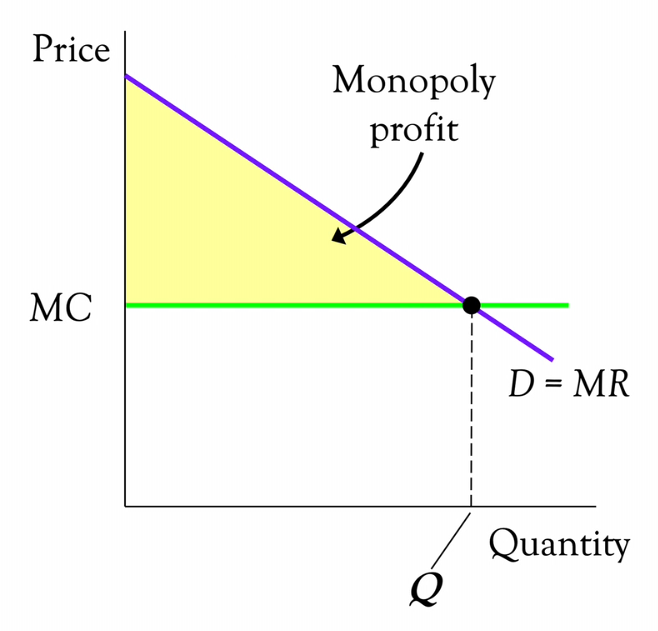
\includegraphics[width=16em]{images/price_discrimination.png}
			\centering
		\end{figure}
	    \item Harford The Undercover Economist Chapter 2: \textit{What Supermarkets Don't Want You to Know}
	    \begin{itemize}
	    	\item Unique target (first-degree)
	    	\begin{itemize}
	    		\item Producer can easily determine consumers' WTP
	    		\item Producer can prevent arbitrage
	    	\end{itemize}
	    	\item Group target (third-degree)
	    	\item Self-incrimination
	    \end{itemize}
	\end{itemize}
\end{itemize}
\subsection{Monopolistic Competition}
\begin{itemize}
	\item \textbf{Many} buyers and sellers
	\item Offer \textbf{differentiated} products
	\item Sellers are \textbf{free} to enter and exit the market
	\begin{itemize}
		\item LR Economic profit = 0 due to entry and exit
		\item New firms enter the market due to existing firms making profits
	\end{itemize}
    \item \impt \textbf{Externalities due to entry of new firms}
    \begin{itemize}
    	\item \textbf{Product-variety externality}: consumers benefit from intro of new products
    	\item \textbf{Business-stealing externality}: existing firms lose revenues when new firms enter the market
    \end{itemize}
\end{itemize}
\subsection{Oligopoly}
\begin{itemize}
	\item \textbf{N-firm Concentration Ratio}: percentage of the market's total output supplied by the N largest firms
	\item Only \textbf{a few} sellers offer similar or identical products
	\item A firm's decision about $P$ or $Q$ can affect other firms
	\begin{itemize}
		\item The firm will consider the reactions from other firms when making decisions
	\end{itemize}
    \item \textbf{Game theory}: study of how people behave in strategic situations
    \item \textbf{Types of oligopoly}
    \begin{itemize}
    	\item \underline{Collusion}: an agreement among firms in a market about quantities to produce or prices to charge
    	\item \underline{Cartel}: A group of firms acting in unison (e.g. price fixing)
    	\begin{itemize}
    		\item Cartel = Monopoly
    		\item Collective firms acting as a single unit, hence graph is equal to monopoly
    	\end{itemize}
    \end{itemize}
\end{itemize}
\subsubsection{Game Theory}
\textbf{Collusion vs self-interest}
\begin{itemize}
	\item Both firms would be better off if they both stick to the cartel agreement
	\item But each firm has an incentive to cheat
\end{itemize}
\textbf{Nash Equilibrium}
\begin{itemize}
	\item A situation in which players interacting with one another each chooses his best strategy given the strategies that all the others have chosen
\end{itemize}
\textbf{Dominant Strategy}
\begin{itemize}
	\item A strategy that is best for a player in a game regardless of the strategies chosen by the other players
\end{itemize}
\textbf{Prisoners' Dilemma}
\begin{itemize}
	\item Cooperation is difficult even when it is mutually beneficial
	\item Both players have dominant strategies that result in inefficient outcomes
	\begin{center}
		\begin{table}[H]
			\centering{
			\begin{tabular}{cc|cc}
				&  & \multicolumn{2}{c}{P2}     \\ \cline{3-4}
				&  & \multicolumn{1}{c|}{A} & B \\ \hline
				\multicolumn{1}{c|}{\multirow{2}{*}{P1}} &
				A &
				\multicolumn{1}{c|}{\begin{tabular}[c]{@{}c@{}}P1: Good\\ P2: Good\end{tabular}} &
				\begin{tabular}[c]{@{}c@{}}P1: Worst\\ P2: Best\end{tabular} \\ \cline{2-4}
				\multicolumn{1}{c|}{} &
				B &
				\multicolumn{1}{c|}{\begin{tabular}[c]{@{}c@{}}P1: Best\\ P2: Worst\end{tabular}} &
				\begin{tabular}[c]{@{}c@{}}P1: Bad\\ P2: Bad\end{tabular}
			\end{tabular}}
		\end{table}
	\end{center}
	\item Non-cooperative oligopoly equilibrium will be
	\begin{itemize}
		\item Bad for oligopoly firms: prevented from achieving \textbf{monopoly} profits
		\item Good for society: $Q$ is closer to the socially efficient output, $P$ is closer to MC
	\end{itemize}
    \item Strategies that lead to cooperation:
    \begin{itemize}
    	\item \textbf{Grim}:\\
    	Initially, a player using grim trigger will cooperate, but as soon as the opponent defects (thus satisfying the trigger condition), the player using grim trigger will defect for the remainder of the iterated game. Since a single defect by the opponent triggers defection forever, grim trigger is the most strictly unforgiving of strategies in an iterated game.
    	\item \textbf{Tit for Tat}\\
    	 For example, two competing economies can use a tit-for-tat strategy so that both participants benefit. One economy \textbf{starts with cooperation }by not imposing import tariffs on the other economy's goods and services to induce good behavior. The idea is that the second economy responds by also choosing not to impose import tariffs. If the second economy reacts by implementing tariffs, the first economy retaliates by implementing tariffs of its own to discourage the behavior.
    \end{itemize}
\end{itemize}

\section{Measurements in Macroeconomics}
\textbf{Origins of Macroeconomics}
\begin{itemize}
	\item Classical economy did not work during the Great Depression
	\item 3 branches:
	\begin{itemize}
		\item \textit{Theory}: John Maynard Keynes
		\item \textit{Policy}: Franklin D Roosevelt
		\item \textit{Measurement}: Simon Kuznets
	\end{itemize}
\end{itemize}
\textbf{Goals in Macro}
\begin{itemize}
	\item \underline{High and sustained economic growth}: Real GDP/GDP Per Capita
	\item \underline{Stable Prices}: CPI
	\item \underline{Low Unemployment}: Employment Rate
\end{itemize}
\subsection{Economic Growth}
Making goods and services (g\&s) that satisfy needs and wants
\begin{itemize}
	\item Goods: tangbible goods
	\item Services: Enjoyed while produced, inseparable from their production
	\item \impt Loan/deposit/cash/shares are not part of g\&s
\end{itemize}
So, \textbf{Economic growth} = rise in an economy's economic production per period\\
\textbf{Why is economic growth desired?}
\begin{itemize}
	\item Required for improvements in living standards and well-being
	\item Provides society with a sense of progress
	\item Helps society avoid conflicts over distribution
\end{itemize}
\subsubsection{GDP}
\textbf{Definition}: \underline{Total monetary value} of \underline{final} goods and services \underline{in a country} \underline{during a given time period}
\begin{itemize}
	\item "Total Monetary value": use current \textbf{market prices}\\
	Indirect measurement of monetary value:
	\begin{itemize}
		\item Financial services: use \textbf{spread}: difference between interest earned on loans and interest paid on deposits
		\item Housing services:\\
		* for tenants, value is measured by \textbf{rent paid}\\
		* For occupiers, value is measured by rent for similar houses
	\end{itemize}
\impt When there are no market prices: e.g. g\&s produced by government for its own use / specialized eqpmt by firms for their own use:
\textbf{estimated by cost of production}
	\item "Final": \textbf{avoid double-counting} goods and services\\
	e.g. Tire used on Ferrari sold to customer is not counted as it is part of a final good (Ferrari)
	\begin{itemize}
		\item Final good: sold to final user
		\item Intermediate good: used up to produce some other good
	\end{itemize}
\item "In a country": inside geographical boundaries (except embassies)
\item "In a given period": Stock vs flow variables, in this case GDP is a flow
\end{itemize}
\subsubsection{Three approaches to measuring GDP}
\begin{enumerate}
	\item \textbf{Expenditure}
	$$Y = C + I + G + NX$$
	\begin{itemize}
		\item \underline{Private consumption}: g\&s purchased by households as final users\\
		\impt C excludes the purchase of new homes, but includes value of housing services enjoyed by both tenants and owner-occupiers\\
		Why?? Might be because of accrual accounting? purchasing 1 big house can be done anytime but
		\item \underline{Private Investment}: g\&s purchased by firms as final users\\
		Include \textbf{capital goods}: goods made to produce other g\&s\\
		Also include \textbf{change in inventories}: goods stored by firms for future use\\
		Also include \textbf{subsidies}
		\item \underline{Government Expenditure}: Expenditure on g\&s by government as final users
		\begin{itemize}
			\item \textbf{Government consumption}: inventory for railroad workers
			\item \textbf{Government investment}: highways, bridges, railroads,
			\item \impt Does not include \textbf{government transfers} to households
		\end{itemize}
	\item \underline{Net Exports}: Exports - Imports
	\end{itemize}
	\item \textbf{Value-added (Production)}
	\begin{equation*}
		\begin{aligned}
\text{A firm's value added} &= \text{Value of g\&s it produces}-\\ &\text{Value of intermediate g\&s it uses up}\\
&= \text{Final} - \text{Initial value}
		\end{aligned}
	\end{equation*}
$$Y = \sum \text{Value-added}$$
This reveals the contribution of various industrial sectors to GDP
	\item \textbf{Income (Income)}
	$$\sum \text{Value-added} = \sum \text{Factor incomes}$$
	\begin{itemize}
		\item A firm's value added is \textbf{paid out} to owners of FOP
		\item Wages = Payments to workers
		\item Interest = Payments to financiers
		\item Rent = Payment to Landlords
		\item Profit = income accruing to firms' owners
	\end{itemize}
\impt: Can tell us distribution of incomes across different factors
\end{enumerate}
\textbf{Comparing GDP across time}
\begin{itemize}
	\item Nominal GDP: GDP at current prices
	\item Real GDP: To make better comparisons of GDP over time
	\item \textbf{Fixed-base approach}
	\begin{itemize}
		\item Choose a base year (arbitrary?!)
		\item Use base year prices to value production for all years
	\end{itemize}
    \item \impt \textbf{Annual Chain-linking approach}
    \begin{itemize}
    	\item \underline{Definition}: Goods and services produced in each year are revalued using the prices of the previous year
    	\item \href{https://www.youtube.com/watch?v=hgbkKn883-U}{Youtube Video}
    	\item Instead of taking an arbitrary year as the base year, we set the last year as the base year
    	\begin{itemize}
    		\item Find growth rate first for each year based on previous year
    		\item To get Real GDP in a given year, chain multiply growth rates from reference year until given year
    		$$RGDP_{i} = RGDP_{k} \times g_{k+1} \times \dots \times g_i$$
    	\end{itemize}
    	\item Limitation: can only compute year-on-year changes of GDP
    	\item Benefits:
    	\begin{itemize}
    		\item Takes into consideration changes in the relative prices of g\&s that occur from one year to the next
    		\item Reflects any recent changes in economic conditions
    	\end{itemize}
    \end{itemize}
\end{itemize}
\textbf{The GDP Deflator}: measure of price level of g\&s included in GDP
$$\text{GDP Deflator} = 100 \times \frac{\text{nominal GDP}}{\text{real GDP}}$$

\subsubsection{Problems with GDP}
\textbf{Quality changes}
\begin{itemize}
	\item Quality should account for more production, but this is subjective
\end{itemize}
\textbf{Free goods and services}
\begin{itemize}
	\item \eg Facebook, Youtube, TikTok
	\item There are associated payments for these but these likely \underline{underestimates} the value of these products
\end{itemize}
\textbf{Shadow Economy/Underground Economy}
\begin{itemize}
	\item informal, illegal, unreported market activities
	\item hard to obtain measurements
	\item Hard to compare GDP across countries if one country has greater importance of the shadow economy
\end{itemize}
\textbf{GDP $\neq$ indicator of well-being}: many important things that matter to well-being are not captured by GDP

\subsection{Price Levels and Inflation}
Note that GDP Deflator is not suitable for measuring changes in households' cost of living (COL) since it includes everything\\
\textbf{Consumer Price Index}
\begin{itemize}
	\item Fix the market basket of g\&s that the average household consumes in a year
	\item Collect prices of items in the market basket for each year
	\item Using the prices, compute the market basket's cost
	\item Choose a base year and compute the CPI and Inflation Rate (year-on-year)
	$$\text{CPI}_\text{current} = 100 \times \frac{\text{CPI}_\text{current}}{\text{CPI}_\text{base}}$$
	\item Real value vs Nominal value
	$$\text{Real Value} = \text{Nominal Value} \times \frac{100}{\text{CPI}}$$
	$$\text{Real i/r} = \text{Nominal i/r} - \text{Inflation Rate}$$
\end{itemize}
\textbf{The Economist Intelligence Unit's Cost of Living Index}
\begin{itemize}
	\item Basket of g\&s = 160 items consumed by expatriate households
	\item Comparison is\underline{ across cities} rather than across time (New York is chosen as base city with index value = 100)
	\item Cost is converted to US Dollars at prevailing exchange rate
\end{itemize}
\subsubsection{Problems with CPI}
\textbf{Upward bias}: \underline{overstates} the amount of inflation the households are experiencing
\begin{itemize}
	\item \textbf{Substitution bias}: when one good increases its price, households tend to switch to cheaper goods but it is not reflected in market basket
	\item \textbf{Outlet bias}: as prices increase, consumers shift purchase from more expensive mainstream stores to cheaper \underline{discount outlets and retailers} but this may be \underline{less represented in statistical authorities' data collection}
	\item \textbf{Quality bias}: inflation does not take into account paying for higher quality
	\item \textbf{New goods bias}:
	\begin{itemize}
		\item New products tend to fall in price and improve in quality during the during the early years of the product's life cycle
		\item However they are only added to the market basket only much later
		\item So CPI fails to capture the fall in price during early years
	\end{itemize}
\end{itemize}

\subsubsection{Stable Prices}
\impt The goal of keeping inflation \textbf{predictable, low, and positive} (2\% per year as a guideline)
\begin{itemize}
	\item Expected inflation can be incorporated into agreements ahead of time, thereby preventing unwanted redistribution of purchasing power
	\begin{itemize}
		\item \eg if inflation rate is higher than predicted, then lender will be worse off and borrower will be better off
		\item \textbf{How to guarantee real inflation rate?}
		\begin{itemize}
			\item Indexation to correct for inflation: loan agreement where
			$$\text{Nominal i/r} = \text{Read i/r} + \text{Inflation rate}$$
			whatever the latter turns out to be
		\end{itemize}
	\end{itemize}
    \item \textit{High inflation} is costly to society
    \begin{itemize}
    	\item \textbf{Distort relative price signals} $\rightarrow$ causing misallocation of resources
    	\item Prompts people to use up valuable resources and time to cope with it
    	\item \textbf{Menu costs}: Sellers change price more often
    	\item \textbf{Shoe leather costs}: costs due to efforts in minimizing money holdings as people go to bank more
    \end{itemize}
    \item \textit{Deflation} is also costly to society
    \begin{itemize}
    	\item \textbf{Definition}: a prolonged spell of negative inflation
    	\item Can make downturns and recessions worse as incomes $\downarrow$
    	\begin{itemize}
    		\item Households and firms postpone purchases to anticipate for lower future prices
    		\item Borrowers incomes fall but their debt and interest may not; \textbf{loan defaults} and \textbf{bankruptcy declarations} increase
    	\end{itemize}
    \end{itemize}
\end{itemize}

\subsection{Low Unemployment}
\textbf{Social costs of having large numbers of unemployed people}:
\begin{itemize}
	\item Labour resources are underutilized
	\item Skills of workers erode with non-use
	\item Health, social, and political problems
\end{itemize}
Ask those \textit{able to work}:
\begin{figure}[H]
	\centering
	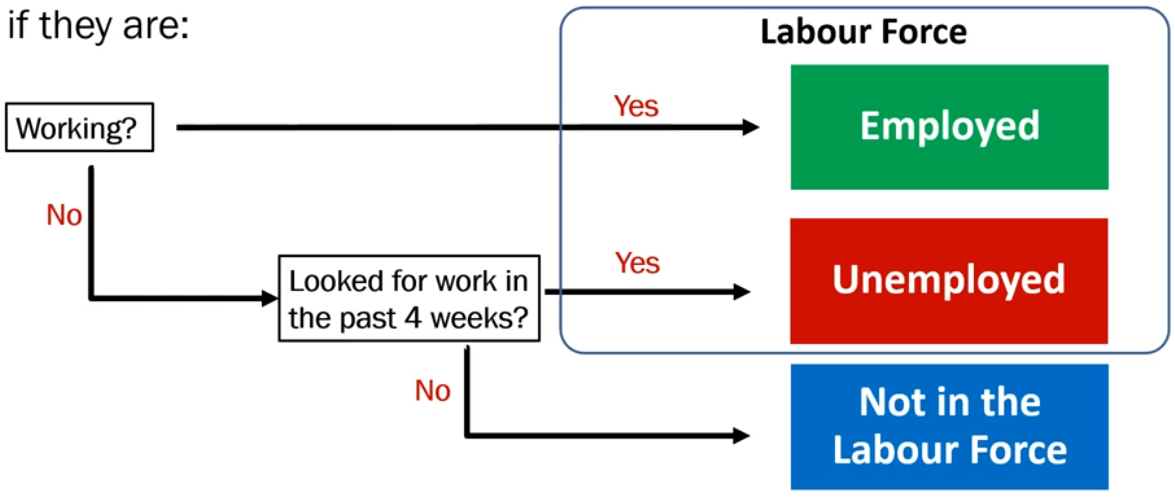
\includegraphics[width=\columnwidth]{images/unemployment.png}
\end{figure}

\begin{equation*}
	\text{Unemployment Rate} = 100\% \times \frac{\text{Unemployed}}{\text{Labour Force}}
\end{equation*}
\begin{equation*}
	\text{Labour Force Participation Rate} = 100\% \times \frac{\text{Labour Force}}{\text{Able to work}}
\end{equation*}
\begin{equation*}
	\text{Employment Rate} = 100\% \times \frac{\text{Employed}}{\text{Able to work}}
\end{equation*}
\begin{figure}[H]
	\centering
	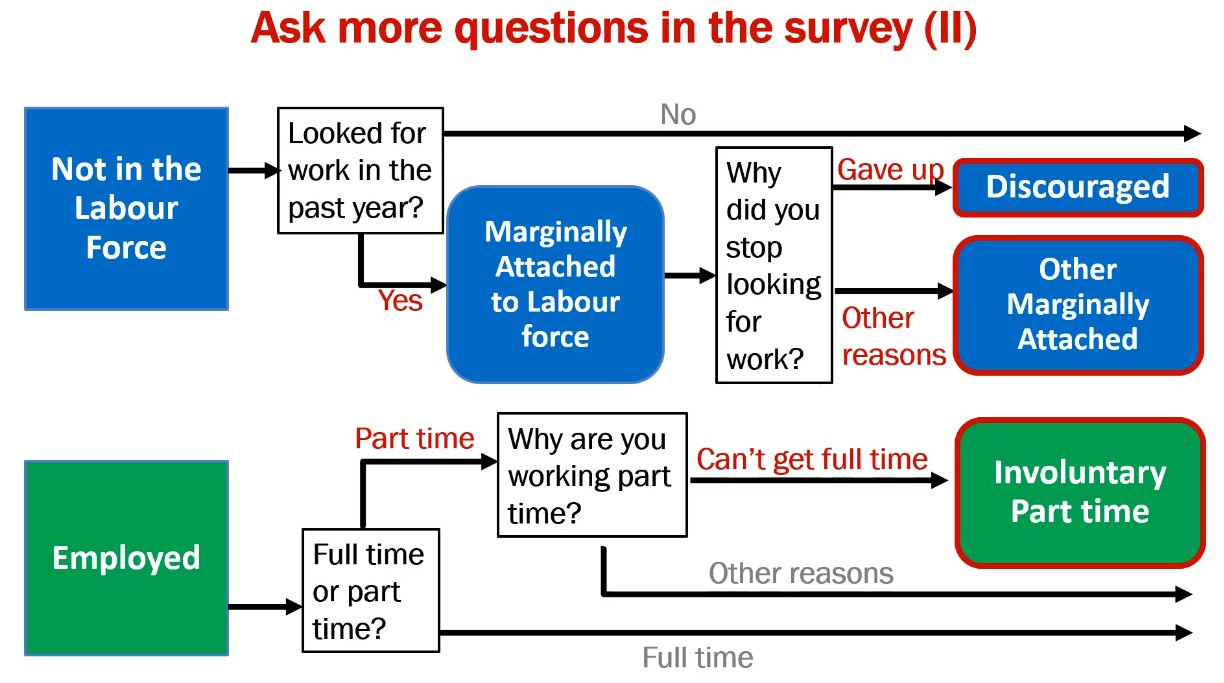
\includegraphics[width=\columnwidth]{images/unemployment2.png}
\end{figure}
\begin{figure}[H]
	\centering
	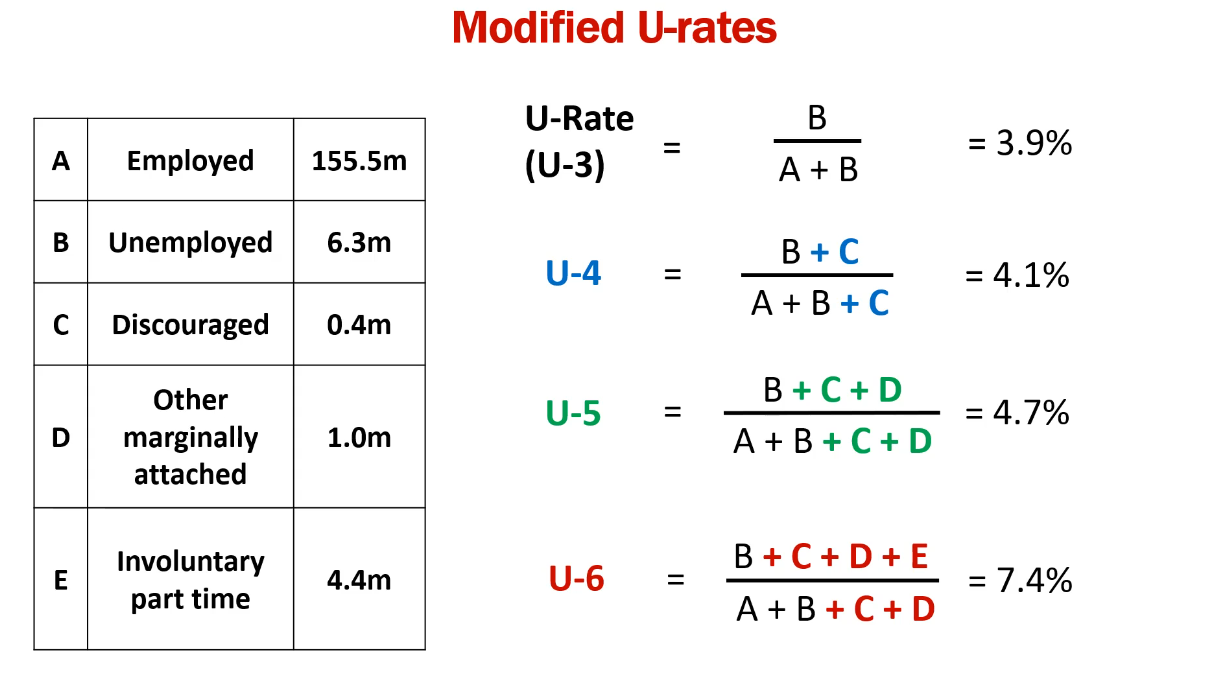
\includegraphics[width=\columnwidth]{images/unemployment3.png}
\end{figure}




\subsubsection{Seasonality in Unemployment}
\begin{itemize}
	\item Short term
	\item Entirely predictable
	\item Seasonally adjusted $\rightarrow$ modified to remove the seasonal variation to facilitate comparisons
\end{itemize}
\subsubsection{Types of Unemployment}
\textbf{Frictional Unemployment}: those in between jobs or just entering labour market
\begin{itemize}
	\item \underline{Characteristics}:
	\begin{itemize}
		\item Looking for good matches
		\item Short term
		\item Generally painless
	\end{itemize}
    \item Government provided unemployment insurance will extend job search time
\end{itemize}
\textbf{Structural Unemployment}:
\begin{itemize}
	\item \underline{Skill mismatch}: mismatch between skills and employers' requirements
	\item \underline{Geographic mismatch}: workers' and employers' locations
	\item \underline{Labour market impediments}: high minimum wage, discrimination, unionization
\end{itemize}
\textbf{Cyclical Unemployment}: fluctuations in unemployment that arises from changes in production over the \textbf{business cycle}
\begin{itemize}
	\item Rise during recessions and fall in between recessions
	\item Note that \textbf{Full employment} refers to \textbf{zero cyclical unemployment} and other types of unemployment are present
	\item At full employment, the output the economy produces is called its \textbf{Potential output}
\end{itemize}

\section{Long-run Macroeconomics}


\subsection{Growth Rate approximation}
\textbf{Rule of 70 approximation:}
$$\text{Time to double} \approx \frac{70}{\text{growth rate percentage point}}$$
\textbf{Approximation for growth rates products and quotients}: let $g_A$ be growth rate of variable $A$
\begin{itemize}
	\item If $C = A \times B$, then $g_C \approx g_A + g_B$
	\item If $C = A / B$, then $g_C \approx g_A - g_B$
\end{itemize}

$$\text{RGDP per capita} = \text{Productivity} \times \text{Avg Hours} \times \text{EPR}$$
$$g_{\text{RGDP per capita}} = g_{\text{Productivity}} + g_{\text{Avg Hours}} + g_{\text{EPR}}$$

\subsection{Divergence}
\textbf{Given sufficient time}, even a \textbf{small difference} in annual growth rate of RGDP creates a \textbf{big difference} in RGDP\\
Why some countries have big growth and others don't?
\begin{itemize}
	\item Institutions needed for markets to thrive must be developed for growth
	\item \eg \textit{Rule of law, market orientation, openness, stability}
\end{itemize}
\subsubsection{Rule of Law}
\begin{itemize}
	\item \textbf{Private property rights}: investment must be secure against \underline{criminal and/or government appropriation}
	\item \textbf{Enforcement of contracts}: Private enforcement is expensive, inefficient and uncertain, much better to rely on a trustable \underline{legal system}
\end{itemize}
\subsubsection{Market Orientation}
Central planning can mobilize resources on massive scale but is prone to \textbf{resource misallocation and mal-investment}
\begin{itemize}
	\item In contrast \textbf{market-based economies} are faster in generating and processing information about needs and constraints
	\item So they are far more adaptive to changes in the economic environment
	\item \textbf{Industrial policy} (govt-directed attempts to grow specific targeted industries) has a mixed record
	\begin{itemize}
		\item They are based on protectionism and will continue to be supported by government without much exposure to the real market, hence inefficient
	\end{itemize}
\end{itemize}
\subsubsection{Openness}
\begin{figure}[H]
	\centering
	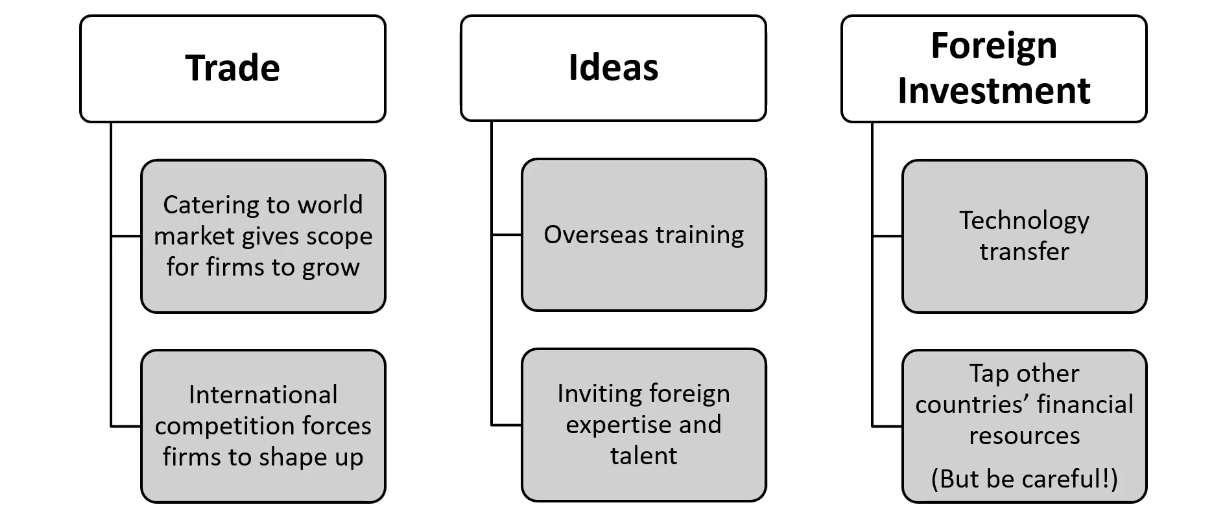
\includegraphics[width=\columnwidth]{images/openness.png}
\end{figure}
\subsubsection{Stability}
\begin{figure}[H]
	\centering
	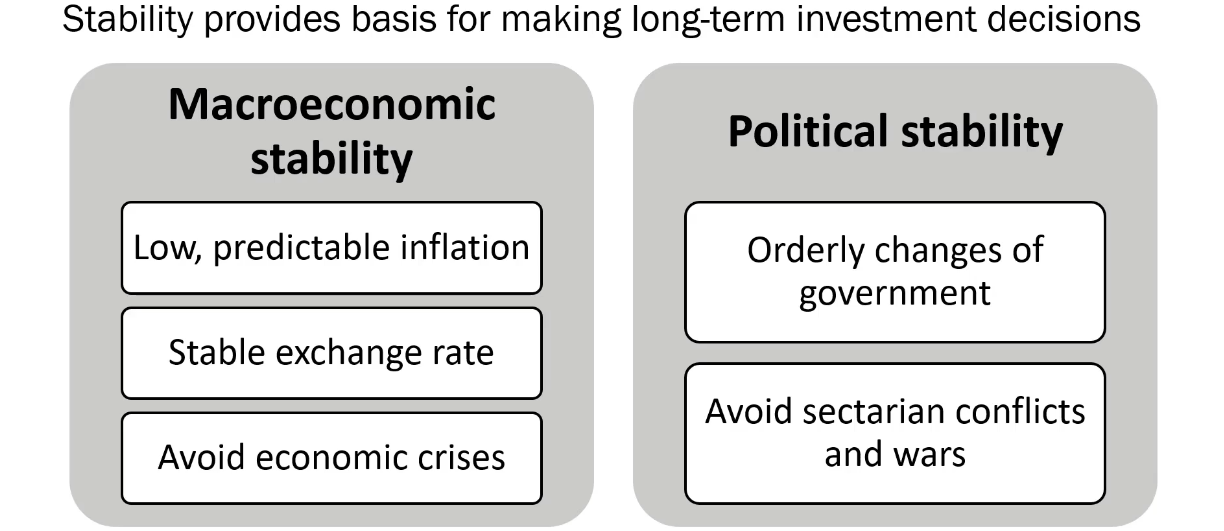
\includegraphics[width=\columnwidth]{images/stability.png}
\end{figure}
\subsection{Aggregate Production}
$$Y = f(L, K, \text{Land}, A)$$
\begin{itemize}
	\item $Y$ is Output
	\item $L$ is Labour
	\item $K$ is Capital
	\item $Land$ is Natural Resources
	\item $A$ is technology
\end{itemize}
\subsubsection{Labour}
For a given $K$ and $A$, if $L$ is doubled, $Y$ would increase by a smaller extent due to \textbf{diminishing returns to labour}
$$g_{\text{RGDP per capita}} = g_{\text{Productivity}} + g_{\text{Avg Hours}} + g_{\text{EPR}}$$
\textbf{Problems with increasing EPR/Avg. hours}:
\begin{itemize}
	\item More labourers will increase Labour Supply (LS) resulting in falling wages and falling household incomes
	\item Encourage \textbf{homemakers} to work: sacrifice child care
	\item Import \textbf{foreign workers}: inability to integrate, loneliness
	\item Encourage \textbf{elderly} to work: not efficient and desirable
	\item \textbf{Lengthen} work hours: Karoshi (death by overwork)
\end{itemize}
So the only effective alternative is to increase productivity (output per unit labour)
$$\frac{Y}{L} = f\left(\frac{K}{L}, A\right)$$

\subsubsection{Capital Deepening}
\textbf{Definition}: raising $K/L$. Assume that $L$ is fixed so raising $K/L$ means raising $K$
$$K_t - K_{t-1} = I_t + G_t - \delta K_t$$
\begin{itemize}
	\item $K_t$ and $K_{t-1}$ are capital stock at time $t$ and $t-1$ respectively, so $K_t - K_{t-1}$(Net Investment) is the change in capital stock (flow variable)
	\item $I_t$ is private investment
	\item $G_t$ is govt investment
	\item $\delta K_t$ is \textbf{Depreciation} (loss due to wear and tear, obsolescence), assumed to be a constant fraction of existing capital stock
\end{itemize}
\textbf{Policies for Capital Deepening}
\begin{enumerate}
	\item Change incentives to \underline{promote investment}
	\begin{itemize}
		\item Reduce corporate tax (on firm's profits) but this effectiveness is mixed
		\item Grant \underline{Investment Tax Credit}: tax reduction for firms that invest in new capital
	\end{itemize}
    \item Change inventives to promote saving
    \begin{itemize}
    	\item Shift from taxing income to taxing consumption
    	\item Reduce transfers to elderly, unemployed
    	\item Mandatory saving (\eg Singapore's CPF)
    \end{itemize}
\end{enumerate}
\textbf{Human Capital}: workers' knowledge, skills, discipline, and health
\begin{itemize}
	\item Increases productivity ($H/L$) but is not included under investment
	\item $H/L$: human capital per unit of labour
	$$\frac{Y}{L} = f\left(\frac{K}{L}, \frac{H}{L},A\right)$$
\end{itemize}
\textbf{Catch-up growth}: poor countries with solid institutional conditions can grow rapidly and catch up with other countries
\begin{itemize}
	\item \eg Post WWII Japan and Germany, Four Asian Tigers
	\item \underline{Elements of catch-up growth}:
	\begin{itemize}
		\item Reduce C, to boost I
		\item Invest in health and education to improve H
		\item Adopt and adapt technology from rest of the world (H and K)
	\end{itemize}
\end{itemize}
\textbf{Limitations of capital deepening}
\begin{itemize}
	\item More K, Less C goods (PPF), but PPF will shift more in the future due to more K goods (legitimate trade-off)
	\item \textbf{Diminishing returns to capital}: productivity growth from capital deepening eventually slows as we increase $K$ (For a given amount of $\bar{L}$ and $\bar{A}$, $Y$ will only increase marginally)
	\item \textbf{Rising depreciation}: as $K$ increases, $\delta K $ will increase and thus \textit{more gross investment is needed to replace depreciated capita;, leaving less for net investment}
\end{itemize}
\subsubsection{Technological Growth}
Productivity growth can come from tech change: \textit{Invention and application of new inputs, new products, or new production methods}
\begin{itemize}
	\item \textbf{Discovery-based growth}: growth based on pushing the technological frontier by creating and using new ideas!
\end{itemize}
\textbf{Some policies:}
\begin{itemize}
	\item \textbf{Intellectual property rights}:
	\begin{itemize}
		\item needed to incentivize commercial R\&D, otherwise copycats can reap gains without paying for R\&D costs (non-rival)
		\item But should not be too strong,otherwise people would be discouraged from using the discovery
		\item Examples:
		\begin{itemize}
			\item \underline{Patent}: right to exclude others from, or charge others for the use of one's invention, valid for a set period
			\item \underline{Copyright}: right to exclude others from, or charge others for, reproducing one's work, valid for a set period
		\end{itemize}
	\end{itemize}
    \item \textbf{Promoting entrepreneurship}: startup culture, seed financing for fledgling entrepreneurship to obtain funding
    \item \textbf{Government funding for R\&D}: Subsidies for private R\&D, government direct funding of R\&D
\end{itemize}
\subsection{Loanable Funds Market}
$$S = I^P + G - T$$
$$Y = C+ I^P + G$$
$$\text{Output} = \text{Planned Spending}$$
\subsubsection{Households}
$$S = Y - T - C$$
\begin{itemize}
	\item $S$ is supply of savings, a portion of $Y$ minus $T$ (net taxes which is Taxes-Subsidies, now is disposable income) minus $C$
	\item \textbf{Determinants of $S$}
	\begin{itemize}
		\item \underline{Real i/r} $\Rightarrow$ if rates increase, it's more lucrative to save
		\item \underline{Future expectations of income}: if Future Y is expected to increase, there will be less $S$ now
		\item \underline{Households wealth}:
	\end{itemize}
\end{itemize}
\subsubsection{Firms}
$$I = I^P + \Delta\text{Inventories}$$
\begin{itemize}
	\item Borrow loanable funds market to finance spending on planned private investment $I^P$
	\item Let all changes in inventories be unplanned
	\item \textbf{Determinants of $I^P$}
	\begin{itemize}
		\item \underline{Real i/r}
		\item \underline{Expected future profits from new capital} (optimism)
	\end{itemize}
\end{itemize}
\subsubsection{Government}
\begin{itemize}
	\item Govt purchases = $G$, Govt collects net taxes $T$
	\item If $G>T $, govt has budget deficit of size $G-T$ and will demand funds
	\item If $T>G$, govt has budget surplus of size $T-G$
	\item \impt Assumption: $G>T$ and always running on budget deficit, and is insensitive to change in real i/r
\end{itemize}
\subsection{The Classical Model}
Focuses on \textbf{resource markets and technology} as \textbf{determinants} of an economy's potential output
\vspace{0.5em}\\
\textbf{Assumption}: \underline{markets clear}:
\begin{itemize}
	\item Labour market reaches equilibrium
	\item Loanable funds market reaches equilibrium
	\item Open vs closed economy?
\end{itemize}
\vspace{0.5em}
\textbf{Say's Law}: "Spending adjusts to equal output (and not the other way around)"
\begin{itemize}
	\item Supply creates its own demand
	\item \textbf{100\% crowding out}: If one spending component increases/falls, output does not change, instead the other spending components fall/increase by the same extent
	\begin{itemize}
		\item Use $Y = C + I^P + G$ at equilibrium and other assumptions (loanable markets, labour market at equilibrium)
	\end{itemize}
\end{itemize}

\section{Short-run Macroeconomics}
\textbf{Singapore's Covid-19 Resilience Package (Fiscal Policy)}
\begin{itemize}
	\item G elements
	\begin{itemize}
		\item Spending on public health and safe reopening
		\item Spending on investments in hardest-hit sectors
	\end{itemize}
    \item T elements
    \begin{itemize}
    	\item Job Support Scheme: paying a portion of workers' salaries
    	\item Recovery Grant: Financial support for workers who lost jobs or were forced to take no-pay leave
    	\item Grants for workers in hardest hit sectors
    \end{itemize}
\end{itemize}
\begin{figure}[H]
	\centering
	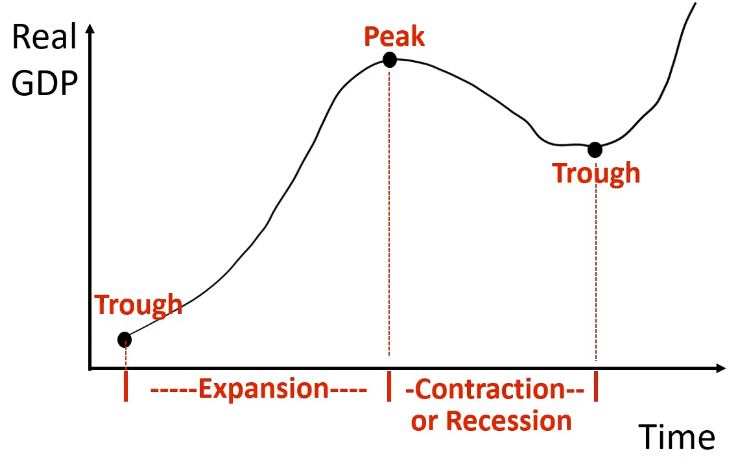
\includegraphics[width=\columnwidth]{images/fluctuations.png}
\end{figure}
\begin{figure}[H]
	\centering
	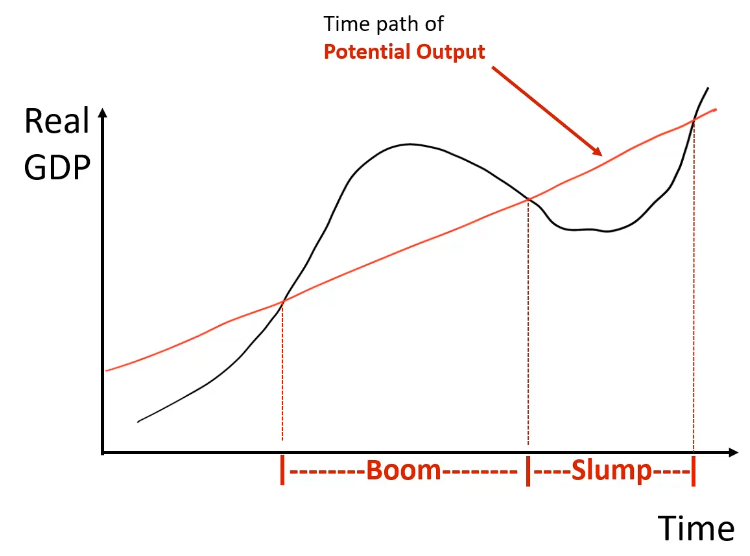
\includegraphics[width=\columnwidth]{images/boomslump.png}
\end{figure}
\textbf{Some terms}: (refer to diagrams)
\begin{itemize}
	\item \textbf{Business Cycles}: another name for econ fluctuations
	\item \textbf{Technical Recession}: two consecutive quarters of contraction (might be abit arbitrary so that's why it's called technical)
	\item \textbf{Boom/Slump}: depends on the position with regards to the economy's \underline{Potential output} (not directly measured and so is estimated)
\end{itemize}
\textbf{What is Short Run Macro?}
\begin{itemize}
	\item LR Macro refers to the time when \underline{all markets clear}, so the Classical Model is a useful guide because the assumptions hold
	\item SR Macro refers to the time period where some markets \underline{do not clear} (Classical Model is not suitable) and economic fluctuations during the period
	\begin{itemize}
		\item \textbf{Labour markets do not clear}: \underline{Sticky Wages assumption holds}
		\begin{itemize}
			\item Wage rates tend to fall slowly, if at all due to inertia, long-term contracts, worries about morale
			\item During recessions, Labour Demand do not usually fall as this will entail a decrease in wages which is not what is observed
			\item Instead, the Sticky Wages assumption holds and so there is a surplus of workers (unemployment) and markets do not clear
		\end{itemize}
		\item \textbf{Loanable funds markets do not clear}:
		\begin{itemize}
			\item Other forces affect i/r, lending and borrowing, especially within relatively shorter time periods
		\end{itemize}
		\item \textbf{Spending depends on output = income}
		\begin{itemize}
			\item The more output produced $\Rightarrow$ more income households receive $\Rightarrow$ more goods and services they purchase
		\end{itemize}
	    \item \textbf{Output depends on spending}
	    \begin{itemize}
	    	\item If spending > output, firms will increase output in response
	    	\item If spending < output, firms will reduce output in response
	    \end{itemize}
	\end{itemize}
\end{itemize}
\subsection{Keynesian Model}
\subsubsection{Spending Depends on Output}
Spending is due to Households ($C$), Firms ($I^P$), Government ($G$), and the External Sector ($NX$) and they are assumed to be \textbf{autonomous} (meaning they do not change when the output $Y$ changes)

$$C = a + b(Y-T), 0<b<1$$
\begin{itemize}
	\item $a$ is the part of consumption independent on disposable income (\textbf{autonomous consumption})
	\item $b(Y-T)$ is part of consumption that depends on disposable income
	\item \textbf{Marginal Propensity to Consume (MPC)}
	$$MPC = \frac{\Delta C}{\Delta Y} = b$$
	\item \textbf{Aggregate Expenditure (AE)}
    $$AE = C + I^P + G + NX$$
    \item \textbf{Demand Shocks}: When AE shifts due to factors that affect $a$, $I^P$, $G$, $T$, and $NX$
    \begin{itemize}
    	\item $a$: expected future income, wealth, real i/r
    	\item $I^P$: business optimism, real i/r
    	\item $G$: fiscal policy decisions
    	\item $NX$: exchange rate, other countries' spending
    \end{itemize}
\end{itemize}
\subsubsection{Output Depends on Spending}
$$I = I^P + \Delta \text{Inventories}$$
\begin{itemize}
	\item $I$ is total investment, $I^P$ is planned investment, change in inventories is assumed to be always unplanned
	\item If $Y>AE$, Inventories will increase as there are unsold goods in the warehouse, $I > I^P$ and Firms will $\downarrow Y$ to $\downarrow$ inventories
	\item If $Y<AE$, Inventories will decrease as firms are producing insufficient g\&s to satisfy spending from parties, $I < I^P$ and Firms will $\uparrow Y$ to $\uparrow$ inventories
	\item Note that firms respond by changing \underline{output}, not \underline{prices} as the economy's price level is assumed to be fixed (short run stickiness in wages and prices)
\end{itemize}
\subsubsection{Goods Market Equilibrium}
Equilibrium is achieved when $Y = AE$ and
$$AE = (a-bT + I^P + G + NX) + bY$$
which is achieved at $Y^*$, the equilibrium level of $Y$
$$Y^* = \frac{1}{1-b}(a-bT + I^P + G + NX)$$
Note that $T=$ Net Taxes = Taxes - Transfers \impt
\begin{figure}[H]
	\centering
	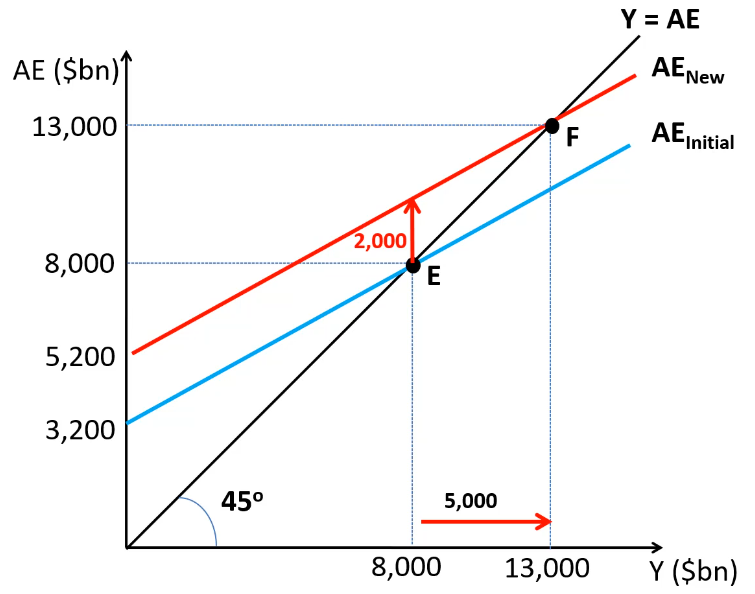
\includegraphics[width=\columnwidth]{images/keynesian.png}
\end{figure}
When there is a change in components ($a$, $I^P$, $G$, or $NX$) due to demand shock, the new equilibrium will increase through \textbf{multiplier process} by
$$\Delta Y^* = \frac{1}{1-b}\Delta I^P \text{ or } G \text{ or } NX$$
\begin{figure}[H]
	\centering
	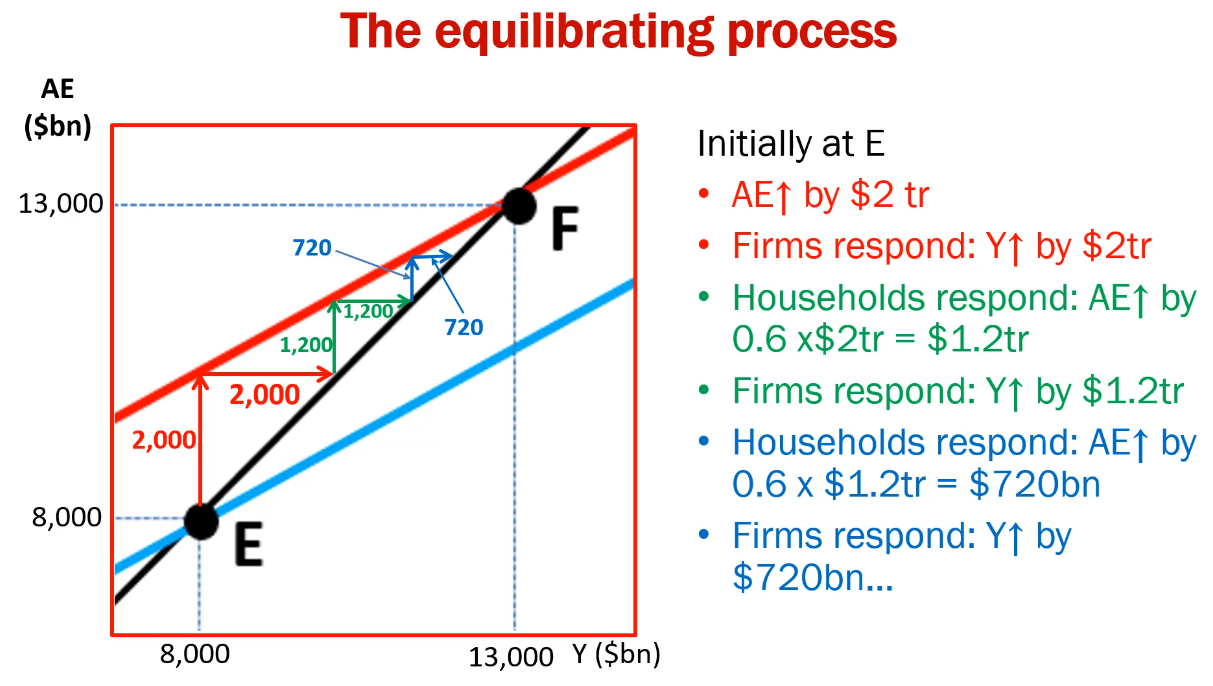
\includegraphics[width=\columnwidth]{images/keynesian_eq.png}
\end{figure}
and $\frac{\Delta Y^*}{\Delta I^P}$, $\frac{\Delta Y^*}{\Delta a}$, $\frac{\Delta Y^*}{\Delta G}$, $\frac{\Delta Y^*}{\Delta NX}$ are called \textbf{expenditure multipliers} and are most of the time given by $\frac{1}{1-b}$
\subsubsection{Explaining Economic Fluctuations}
\begin{itemize}
	\item Fluctuations are mostly due to \textbf{demand shocks}, which are amplified by the multiplier process
	\item Main sources of demand shocks
	\begin{itemize}
		\item $I^P$ is the most volatile because it depends on business optimism and expectations which are volatile (animal spirits)
		\item For small open economies, $NX$ can be highly volatile
	\end{itemize}
    \item There is no relationship between equilibrium output ($Y^*$) and potential output ($Y_{FE}$), as the economy can be in a slump or a boom for a protracted period of time
    \begin{itemize}
    	\item Output gap = $Y^* - Y_{FE}$
    	\item Percentage output gap = $100\% \times \frac{Y^* - Y_{FE}}{Y_{FE}}$
    \end{itemize}
\end{itemize}

\subsubsection{Automatic Stabilizers and Destabilizers}
\begin{itemize}
	\item \textbf{Automatic stabilizers}: features of the economy that automatically dampen the spending resposne during the multiplier process
	\begin{itemize}
		\item makes the multiplier smaller
		\item makes the economy more stable in the short run
	\end{itemize}
	\item \textbf{Automatic destabilizers}: features of the economy that automatically strengthen the spending resposne during the multiplier process
	\begin{itemize}
		\item makes the multiplier bigger
		\item makes the economy less stable in the short run
	\end{itemize}
\end{itemize}
Suppose there is a positive demand shock and $Y \uparrow$
\begin{itemize}
	\item Relax the assumption that $T$ is autonomous
	\begin{itemize}
		\item When $Y \uparrow$, there will be increase in income tax revenue, sales tax revenue, and decrease in trasnfers to unemployed \& poor (overall increase in $T$)
		\item $T \uparrow$ means $C\downarrow$ and this partially \textbf{counteracts} the initial $Y\uparrow$
	\end{itemize}
	\item Relax the assumption that $M$ (imports) are autonomous
	\begin{itemize}
		\item When $Y \uparrow$, $C \uparrow$ and more of this is spent on purchasing imports
		\item Hence the multiplier becomes smaller
	\end{itemize}
    \item Household wealth may rise with income
    \begin{itemize}
    	\item Stock prices, prices of homes rise rapidly during booms
    	\item When $Y\uparrow$, $a \uparrow$ which means $a$ is not autonomous
    \end{itemize}
    \item Planned investment ($I^P$) may rise with income as firms become more optimistic as economy booms
\end{itemize}

\subsubsection{Keynesian vs Classical}
In the \underline{Keynesian model}, spending depends on output so an increase in $S$ will lead to a fall in $Y$ and so on and so forth which is not good for the economy (\textbf{The Paradox of Thrift})\\
In the \underline{Classical model}, spending adjusts to output $\Rightarrow$ an increase in $S$ will be counteracted by a fall in $I^P$ (Say's Law) so Y remains unchanged

\subsection{Countercyclical Fiscal Policy}
\textbf{Definition}: fiscal policy aiming to dampen economic fluctuations
\begin{itemize}
	\item If $Y^* < Y_{FE}$, countercyclical FP should be \textbf{expansionary} (Aim to $\uparrow AE$ by $\uparrow G$ or $\downarrow T$)
	\item If $Y^* > Y_{FE}$, countercyclical FP should be \textbf{contractionary} (Aim to $\downarrow AE$ by $\downarrow G$ or $\uparrow T$)
	\item By contrast, \textbf{fiscal austerity} during a slump is \textbf{procyclical}
\end{itemize}
To counter a slump, $G$ only needs to be a fraction of the output gap to close the gap and reach $Y_{FE}$, in contrast, we need bigger change in $T$ as a change in $T$ only affects a portion of $Y$
$$\text{G-Multiplier} = \frac{\Delta Y^*}{\Delta G} = \frac{1}{1-MPC}$$
$$\text{T-Multiplier} = \frac{\Delta Y^*}{\Delta T} = -MPC \times \frac{1}{1-MPC}$$
\impt in SG, $G$ is pegged to a seven-year moving average of past and projected GDP to reduce volatility in $G$ spending
\subsubsection{Problems with FP}
\textbf{Timeliness Problem}: discretionary FP prone to lags since time is used to
\begin{itemize}
	\item Collect and interpret macroeconomic data
	\item Formulate the fiscal plan
	\item Get legislative approval for the spending plan
\end{itemize}
\textbf{Irreversibility Problem}
\begin{itemize}
	\item Ideally counter-cyclical policy should be reversible (should be able to withdraw stimulus after recovery)
	\item But it is difficult to reverse
	\begin{itemize}
		\item Voters hate $T \uparrow$ again and $G_{\text{transfers}} \downarrow$
		\item Businesses that benefit from $G$ will lobby the govt to keep spending
	\end{itemize}
\end{itemize}
\textbf{Monetary Policy is available}
\begin{itemize}
	\item Central Bank may already have used monetary policy to stabilize the economy which is fast and easy to reverse
	\item Central banks are usually independent from govt, to insulate monetary policy from political considerations
\end{itemize}
\textbf{Theory vs Practice}
\begin{itemize}
	\item Size of \underline{output gap}: cannot be estimated accurately
	\item Size of \underline{multiplier}: uncertainty about size
	\item Size of \underline{stimulus}: political considerations dominate (govt wants to appease as many people as possible, big stimulus would anger some people)
	\item \underline{Mix} of G\&T: similar to above (political considerations)
	\item \underline{Timing} of stimulus: ideally applied ASAP, but there is always time lag
\end{itemize}
\textbf{Leakages and Savings}
\begin{itemize}
	\item Effectiveness of FP is more limited for open economies due to $M$ leakages
	\item Fiscal transfer effect would be blunted if the economy has a high $S$ savings rate because injections are not fully spent, but instead kept as precautionary savings
\end{itemize}
\textbf{Fiscal Sustainability: trading off long-term investments}
\begin{itemize}
	\item Large deficits necessitates the government to borrow, which increases interest rates and \underline{crowd out} funds for private investments
	\item This will reduce long-term growth prospects
	\item However in Singapore, budget deficits is always financed from past year surplus
\end{itemize}
\subsubsection{Singapore's Countercyclical FP in 2020}
\begin{itemize}
	\item \underline{Jobs Support Scheme}: \$20 billion wage subsidy
	\begin{itemize}
		\item Able to support businesses wage expenses and prevent retrenchment
	\end{itemize}
    \item \underline{Covid-19 Support Grant}: discretionary unemployment benefit
    \item \underline{Care and Support Package}:
    \begin{itemize}
    	\item Vouchers for groceries, utilities, and conservancy
    	\item Poorer families get more
    \end{itemize}
    \item \underline{Solidarity payment}: cash transfers to citizens and PR
    \item \underline{Government-sponsored traineeships}: to reduce unemployment spell for those entering job market
    \item \underline{Industry-specific help}: \$100 credit per household to use on local tourism $\Rightarrow$ \impt improve business expectations and demand, reduce precautionary savings inclination that can dampen consumption
\end{itemize}

\section{Money and Banking}
\subsection{Money}
\textbf{Functions of money}
\begin{itemize}
	\item \underline{Medium of exchange}: without money, people have to barter, but each party has to desire the other party's good
	\item \underline{Unit of account}: measuring stick for valuing g\&s, assets, liabilities on a common basis, also needed to record values
	\item \underline{Store of value}: keep money today to be spent in the future (an asset part of people's asset portfolios)
\end{itemize}
\textbf{Money history}
\begin{itemize}
	\item \textbf{Commodity as money}: For most of history, commodities were used as money, with their \underline{intrinsic value} as an \underline{exchange value}
	\item \textbf{Commodity-backed money}: Certificates representing a claim on commodity in storage
	\begin{itemize}
		\item More convenient than carrying commodity around
		\item Example would be bank issued \underline{bank notes} for gold and silver deposits
	\end{itemize}
    \item \textbf{Fiat Money}: value of fiat money depends on peoples' willingness to accept it in payment
    \begin{itemize}
    	\item Govt can decree a currency to be \textbf{legal tender} (recognize by law as valid for payments), but ultimately it's up to people to accept it
    \end{itemize}
\end{itemize}
\textbf{Monetary aggregates}
\begin{itemize}
	\item \textbf{M1}: greatest \underline{liquidity}: assets can be sold quickly for currency, with as little impact on its selling price
	\begin{itemize}
		\item \textbf{Currency in circulation}: excludes cash in bank vaults and ATMS
		\item \textbf{Demand deposits/Checking Deposits}: deposits that are used for making transactions
	\end{itemize}
    \item \textbf{M2} = M1 + very liquid assets
    \item \textbf{M3} = M1 + liquid assets
\end{itemize}

\subsection{Banks}
\begin{figure}[H]
	\centering
	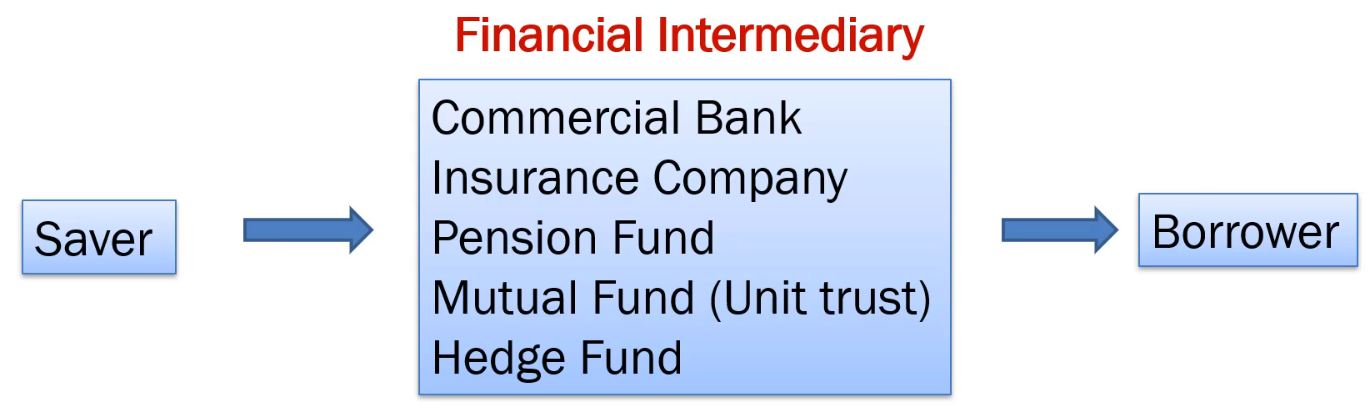
\includegraphics[width=\columnwidth]{images/fin_intermediaries.png}
\end{figure}
\textbf{Financial Intermediaries}
\begin{itemize}
	\item Get money from savers, and the money is in turn invested/lent to borrowers
	\item Earn profit by charging a \textbf{spread} between i/r they pay to savers and i/r they obtain from borrowers
	\item Benefits of finanical intermediaries
	\begin{itemize}
		\item \underline{Expertise at evaluating and monitoring borrowers}: need to know if the borrower has good/bad risk
		\item \underline{Ability to finance large projects}: bank pools funds from many savers as compared to needing many people if need to borrow individually
		\item \underline{Low risk to saver}: the risk is diversified across many borrowers
		\item \underline{Liquidity for savers}: Bank deposits are liquid as opposed to loans from individuals which are \textit{bound by contract} (cannot be converted into cash readily)
	\end{itemize}
\end{itemize}
\textbf{Financial Markets}
\begin{itemize}
	\item Where lending and borrowing of funds are conducted
	\begin{itemize}
		\item \eg market for bank loans, and organized markets where securities (tradable financial instruments) are bought and sold
		\item \eg \textbf{Stocks}: represent claim in equity and ownership of a company; Stock exchange (secondary market) and IPO (primary market)
		\item \eg \textbf{Bonds} in bond market: a tradable debt security representing a promise to repay borrowed funds
	\end{itemize}
\end{itemize}
\textbf{Banks}
\begin{itemize}
	\item Balance sheet:
	\begin{itemize}
		\item \underline{Assets} comprises of Cash in Vault and ATMS and Deposits at the Central Bank
		\item \underline{Liabilities}: Demand Deposits
		\item \underline{Equity}: Bank Capital
	\end{itemize}
\end{itemize}


\subsubsection{Money Multiplier (Money Creation)}
\textbf{Assumption}:
\begin{itemize}
	\item RRR = 10\%
	\item Banks do not want to hold excess reserves
	\item \textbf{Cashless society}, with money held only in the form of bank deposits
	\item Bank reserves are composed entirely of deposits at the Central Bank
\end{itemize}
\textbf{Process}
\begin{enumerate}
	\item Central Bank buys bond from the government, reserves (assets) and deposits (liabilities) of the first bank increases
	\item Since RRR is 10\%, the remaining 90\% of the reserves is loaned to another individual using a different bank
	\item Second bank gets 90\% of original amount of reserves, and the process continues
	\item \textbf{Money Multiplier}: amount of money created (or destroyed) for each dollar of reserves injected (or withdrawn)
	$$\text{Money Multiplier} = \frac{1}{\text{RRR}}$$
	\item In practice, the multiplier could be smaller than $\frac{1}{\text{RRR}}$ because
	\begin{itemize}
		\item Banks may hold excess reserves $\rightarrow$ actual reserves ratio is higher than RRR
		\item People may hold part of money as cash (cashless assumption is not held)
	\end{itemize}
\end{enumerate}
\subsection{Central Bank}
\begin{itemize}
	\item Independent from government
	\item Not allowed to print money to make transfers or to purchase goods and services (since it can lead to hyperinflation (50\% sustained inflation rate))
	\item \textbf{Objectives}
	\begin{itemize}
		\item Ensure financial stability
		\item Conduct monetary policy for price stability and/or managing economic fluctuations
	\end{itemize}
	\item \textbf{Role of Central Bank in banking}
	\begin{itemize}
		\item \underline{Bank for commercial banks}: banks keep most of their reserves in the form of deposits with the central bank
		\begin{figure}[H]
			\centering
			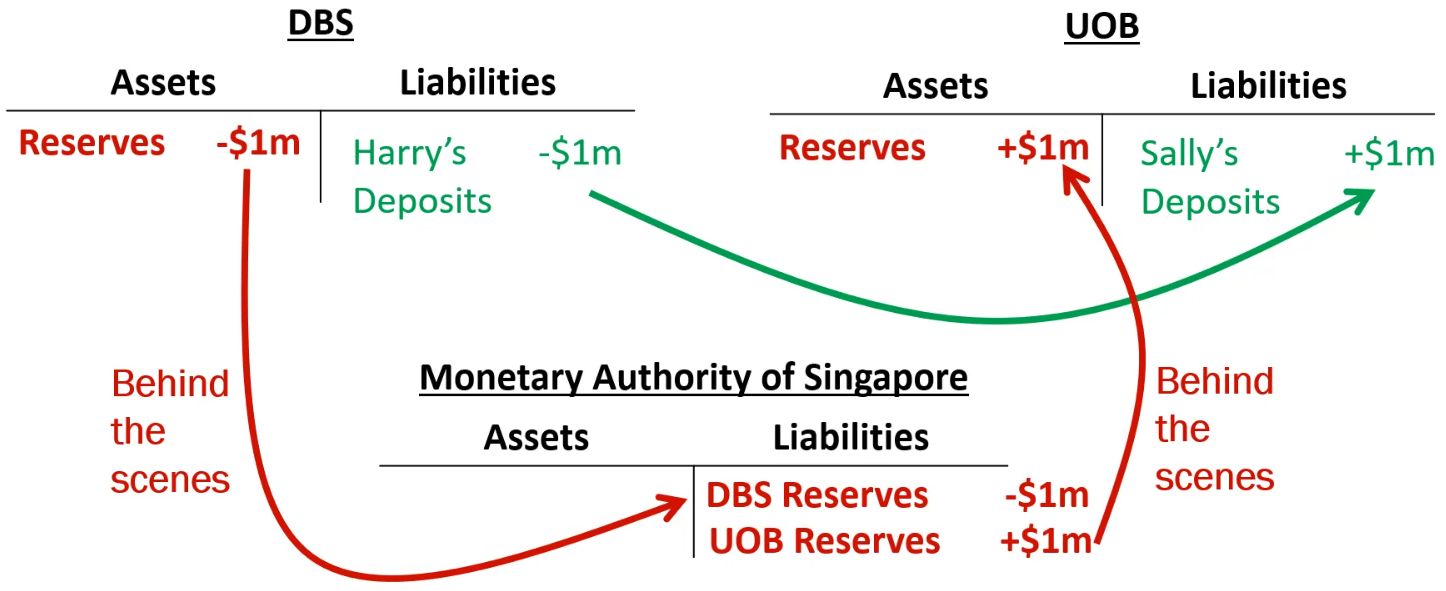
\includegraphics[width=\columnwidth]{images/centralbank.png}
		\end{figure}
		\item \underline{Regulator of banks and fin institutions}
		$$\text{Reserve Ratio} = \frac{\text{Reserves}}{\text{Demand Deposits}}$$
		Many central bank impose minimum reserve requirements which is the \textbf{Required Reserve Ratio} (RRR)
		\begin{itemize}
			\item Banks can choose to hold excess reserves
			\item If banks are short of reserves, they can (1) attract deposits, (2) recall loans or sell other assets, (3) borrow reserves from other banks or from the Central Bank
		\end{itemize}
	\end{itemize}

\end{itemize}
\subsubsection{Central Bank's Role in Money Creation}
\begin{enumerate}
	\item \textbf{Changing RRR}
	\begin{itemize}
		\item $\uparrow$RRR $\Rightarrow$ Loans$\uparrow$, Deposits$\uparrow$
		\item $\downarrow$RRR $\Rightarrow$ Loans$\downarrow$, Deposits$\downarrow$
	\end{itemize}
    \item \textbf{Open Market Operations}: change the quantity of reserves by purchasing or selling short-term \underline{government securities}
    \begin{itemize}
    	\item Open Market Purchase $\Rightarrow$ Reserves$\uparrow$, Loans$\uparrow$, Deposits$\uparrow$
    	\item Open Market Sale $\Rightarrow$ Reserves$\downarrow$, Loans$\downarrow$, Deposits$\downarrow$
    \end{itemize}
    \item \textbf{Discount loans}: Banks that are short of reserves can take a discount loan from the Central Bank
    \begin{itemize}
    	\item \textbf{Discount rate} = interest rate on discount loan
    	\item Reduce discount rate $\Rightarrow$ Banks can have bigger reserves and this bigger reserves can be used for loans $\Rightarrow$ Reserves$\uparrow$, Loans$\uparrow$, Deposits$\uparrow$
    	\item Raise discount rate $\Rightarrow$ Reserves$\downarrow$, Loans$\downarrow$, Deposits$\downarrow$
    \end{itemize}
    \item \textbf{Changing the i/r paid on reserves}: changes banks' willingness to make loans and reserves
    \begin{itemize}
    	\item $\downarrow$i/r $\Rightarrow$ encourages bank to make more loans, Loans$\uparrow$, Deposits$\uparrow$
    	\item $\uparrow$i/r $\Rightarrow$ encourages bank to make fewer loans, Loans$\downarrow$, Deposits$\downarrow$
    \end{itemize}
\end{enumerate}
\subsubsection{Central Bank's Role in Stability}
\textbf{Banks are inherently fragile}
\begin{itemize}
	\item In making loans, they create money
	\item Bank failures can damage the functioning of the economy
	\item Banks are fragile because
	\begin{itemize}
		\item Highly \textbf{leveraged}: using borrowed funds to buy assets
		$$\text{Leverage Ratio} = \frac{\text{Assets}}{\text{Equity}}$$
		$$\text{Capital Ratio} = \frac{\text{Equity}}{\text{Assets}}$$
		Leverage amplifies losses and gains (if assets change, the equity will change drastically assuming liabilities is constant and A = L+E)$\Rightarrow$ easy for banks to get \textbf{insolvent}: cannot pay off its liabilities even if it sells all its assets
		\item "borrow short" and "lend long"
	\end{itemize}
\end{itemize}
\textbf{Bank Runs}
\begin{itemize}
	\item \textbf{Bank runs}: If depositors suspect a bank to be insolvent, they will rush to withdraw deposits
	\item Deposits are \underline{short term} liabilities and can be withdrawn anytime, but banks DO NOT have the reserves to handle massive deposit withdrawals
	\item Banks need to convert non-current assets such as loans to short-term and relatively more liquid assets
	\item So bank will have to shut down
	\item \textbf{Bank panic}: depositors become suspicious about health of other banks so many banks will have to shut down
	\begin{itemize}
		\item Payment systems are disrupted
		\item Wealth is destroyed
		\item Lack of bank lending
	\end{itemize}
\end{itemize}
\textbf{Policies for Financial Stability}: to prevent banking runs
\begin{itemize}
	\item \underline{Reserve requirements}: RRR
	\item \underline{Capital requirements}: minimum capital ratio to reduce leverage
	\item \underline{Restricting bank's activities}, regular monitoring
	\item \underline{Deposit insurance}: mandatory provided by government to prevent runs and panics
	\begin{itemize}
		\item Banks pay premiums to the SDIC (Singapore Deposit Insurance Corporation)
		\item If there is a bank run and the bank cannot pay depositors, SDIC will pay on its behalf
		\item Deposit insurance removes the sense of urgency to withdraw deposits, preventing bank runs from happening
	\end{itemize}
    \item \underline{Lender of last resort}: central banks lend to troubled banks when no one else will
    \item \underline{Owner of last resort}: Central banks/govt inject funds to boost bank capital
\end{itemize}
\end{multicols}










\end{document}